\documentclass[aspectratio=169]{beamer}
\usetheme{Madrid}
\usecolortheme{seahorse}
\usepackage{amsmath}
\usepackage{amssymb}
\usepackage{tikz}
\usepackage{algorithm}
\usepackage{algpseudocode}
\usepackage{xcolor}
\usepackage{tcolorbox}
\usepackage{pgfplots}     % This automatically loads the 'tikz' package
\pgfplotsset{compat=1.18} % Good practice for pgfplots
\usepackage{amsmath}      % For the 'align*' environment
\usetikzlibrary{shapes.geometric, arrows.meta, positioning, calc, patterns}
\usepackage{pifont}           % Provides the dingbat symbols like \ding{55}
\usepackage{newunicodechar}   % Allows you to define Unicode characters
\newunicodechar{✓}{\checkmark}
\newunicodechar{✗}{\ding{55}}
% Custom colors
\definecolor{highDcolor}{RGB}{46, 134, 171}
\definecolor{lowDcolor}{RGB}{162, 59, 114}
\definecolor{gradcolor}{RGB}{255, 127, 14}

% Add these color definitions in the preamble (after line 16)
\definecolor{gray30}{gray}{0.3}
\definecolor{gray50}{gray}{0.5}
\definecolor{gray70}{gray}{0.7}

% Custom commands
\newcommand{\conceptbox}[2]{\colorbox{#1!20}{\textcolor{#1}{\textbf{#2}}}}
\newcommand{\warning}[1]{\conceptbox{red}{Warning: #1}}
\newcommand{\insight}[1]{\conceptbox{blue}{Insight: #1}}
\newcommand{\ethics}[1]{\conceptbox{purple}{Ethics: #1}}

\title{t-Stochastic Neighbor Embedding}
\subtitle{Complete 80-Slide Presentation}
\author{Prof.Asc. Endri Raco}
\institute{Polytechnic University of Tirane}
\date{October 2025}

\begin{document}

% ============================================
% SLIDES 1-10: Introduction and Fundamentals
% ============================================

% Slide 1
\begin{frame}
\titlepage
\end{frame}

% =================================================================
% REVISED NEW SLIDE 1 (v5): FINAL COMPACT LAYOUT
% =================================================================
\begin{frame}{What is High-Dimensional Data? An Intuitive View}
    \begin{block}{The Core Idea}
        Think of data not as a spreadsheet, but as points in a "feature space." Each feature is a dimension.
    \end{block}

    \begin{columns}[T]
        \column{0.45\textwidth}
            \textbf{Simple Example: Housing Prices (2D)}
            \begin{itemize}\small
                \item Dimension 1: Square Footage
                \item Dimension 2: Price
                \item \textit{Easy to plot and see patterns!}
            \end{itemize}

            \vspace{0.4cm} % Further reduced vertical space
            \textbf{Complex, High-Dimensional Examples:}
            \begin{itemize}\small
                \item \textbf{An Image (784-D):} Each pixel's brightness is one dimension.
                \item \textbf{A Customer (100s of D):} Dimensions for age, purchase history, clicks...
                \item \textbf{A Document (1000s of D):} Each dimension is a word's count.
            \end{itemize}

        \column{0.55\textwidth}
            \begin{center}
            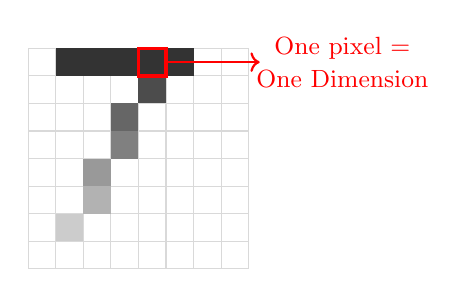
\begin{tikzpicture}[scale=0.7] % Further reduced scale
                \begin{scope}
                    \draw[gray!30, thin, step=0.5] (-2,-2) grid (2,2);
                    \fill[black!80] (-1.5,1.5) rectangle (-1,2);
                    \fill[black!80] (-1,1.5) rectangle (-0.5,2);
                    \fill[black!80] (-0.5,1.5) rectangle (0,2);
                    \fill[black!80] (0,1.5) rectangle (0.5,2);
                    \fill[black!80] (0.5,1.5) rectangle (1,2);
                    \fill[black!70] (0,1) rectangle (0.5,1.5);
                    \fill[black!60] (-0.5,0.5) rectangle (0,1);
                    \fill[black!50] (-0.5,0) rectangle (0,0.5);
                    \fill[black!40] (-1,-0.5) rectangle (-0.5,0);
                    \fill[black!30] (-1,-1) rectangle (-0.5,-0.5);
                    \fill[black!20] (-1.5,-1.5) rectangle (-1,-1);
                    \draw[red, very thick] (0,1.5) rectangle (0.5,2);
                    \node[text=red, align=center] at (3.7, 1.75) {\small One pixel = \\ \small One Dimension};
                    \draw[->, red, thick] (0.5,1.75) -- (2.2,1.75);
                \end{scope}
            \end{tikzpicture}
            
            \begin{tcolorbox}[colback=yellow!10, colframe=orange!60, boxrule=1pt, width=\linewidth, top=1mm, bottom=1mm] % Added top/bottom padding control
                \centering\small
                \textbf{Key Idea:} We often work with data that has far more dimensions than the 2 or 3 we can perceive. This creates unexpected problems.
            \end{tcolorbox}
            \end{center}
    \end{columns}
\end{frame}


\begin{frame}{What is Dimensionality Reduction?}
\begin{block}{Definition}
Transforming high-dimensional data into lower-dimensional representations while preserving meaningful structure
\end{block}

\textbf{Why We Need It:}
\begin{itemize}
\item Visualization: Human perception limited to 3D
\item Curse of dimensionality: Distance becomes meaningless in high-D
\item Computational efficiency: Reduce processing requirements
\item Feature extraction: Identify essential patterns
\end{itemize}

\textbf{The Central Challenge:}
\begin{center}
\Large How do we decide what to preserve when we must lose information?
\end{center}

\begin{columns}
\column{0.5\textwidth}
\centering
Traditional answer: \textcolor{blue}{Preserve distances}

\column{0.5\textwidth}
\centering
t-SNE answer: \textcolor{red}{Preserve neighborhoods}
\end{columns}
\end{frame}

% Slide 2
\begin{frame}{The Fundamental Challenge of Dimensionality Reduction}
\begin{columns}
\column{0.5\textwidth}
\begin{center}
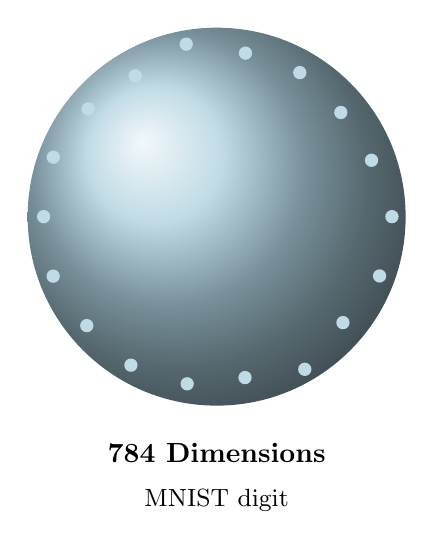
\begin{tikzpicture}[scale=1.2]
\shade[ball color=highDcolor!40] (0,0) circle (2cm);
\foreach \angle in {0,20,...,340} {
    \pgfmathsetmacro\radius{1.7+0.2*rnd}
    \fill[white!70!highDcolor] (\angle:\radius) circle (2pt);
}
\node at (0,-2.5) {\textbf{784 Dimensions}};
\node at (0,-3) {\small MNIST digit};
\end{tikzpicture}
\end{center}

\column{0.5\textwidth}
\begin{center}
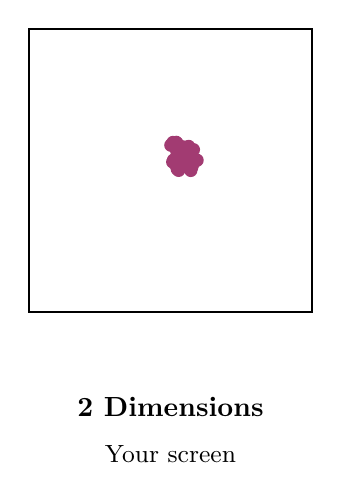
\begin{tikzpicture}[scale=1.2]
\draw[thick] (-1.5,-1.5) rectangle (1.5,1.5);
\foreach \i in {1,...,30} {
    \pgfmathsetmacro\x{0.3*rnd}
    \pgfmathsetmacro\y{0.3*rnd}
    \fill[lowDcolor] (\x,\y) circle (2pt);
}
\node at (0,-2.5) {\textbf{2 Dimensions}};
\node at (0,-3) {\small Your screen};
\end{tikzpicture}
\end{center}
\end{columns}

\vspace{0.5cm}
\begin{center}
\Large\textbf{How do we preserve neighborhood relationships \\ when destroying geometric structure?}
\end{center}
\end{frame}


% Slide 3
\begin{frame}{The Crowding Problem: Why Linear Methods Fail}
\begin{block}{Definition}
\textbf{Crowding Problem:} The geometric impossibility of preserving moderate-range distances when projecting from high to low dimensions, causing distinct distance scales to collapse.
\end{block}

\begin{columns}
\column{0.5\textwidth}
\begin{center}
\textbf{High-D Space (10D)}\\[0.2cm]
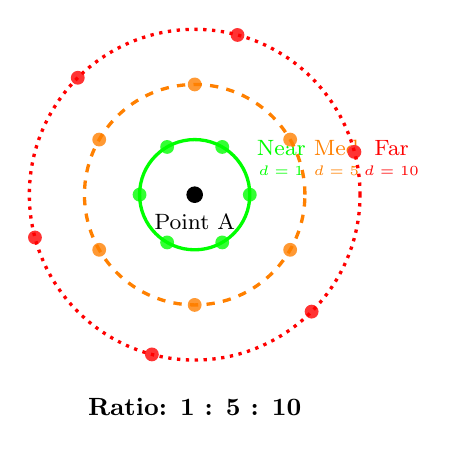
\begin{tikzpicture}[scale=1.0]
% Center point
\fill[black] (0,0) circle (3pt);
\node at (0,-0.35) {\footnotesize Point A};

% Near neighbors (distance = 1)
\foreach \angle in {0,60,120,180,240,300} {
    \fill[green!80] (\angle:0.7) circle (2.5pt);
}
\draw[green, very thick] (0,0) circle (0.7);
\node[green] at (1.1,0.6) {\footnotesize Near};
\node[green] at (1.1,0.3) {\tiny $d=1$};

% Moderate neighbors (distance = 5)
\foreach \angle in {30,90,150,210,270,330} {
    \fill[orange!80] (\angle:1.4) circle (2.5pt);
}
\draw[orange, very thick, dashed] (0,0) circle (1.4);
\node[orange] at (1.8,0.6) {\footnotesize Med};
\node[orange] at (1.8,0.3) {\tiny $d=5$};

% Far neighbors (distance = 10)
\foreach \angle in {15,75,135,195,255,315} {
    \fill[red!80] (\angle:2.1) circle (2.5pt);
}
\draw[red, very thick, dotted] (0,0) circle (2.1);
\node[red] at (2.5,0.6) {\footnotesize Far};
\node[red] at (2.5,0.3) {\tiny $d=10$};

\node at (0,-2.7) {\small\textbf{Ratio: 1 : 5 : 10}};
\end{tikzpicture}
\end{center}

\column{0.5\textwidth}
\begin{center}
\textbf{After Linear Projection to 2D}\\[0.2cm]
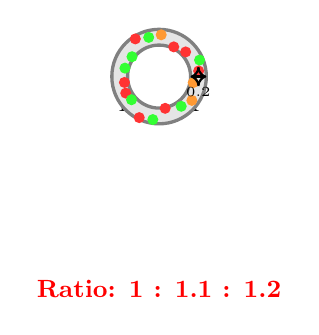
\begin{tikzpicture}[scale=1.0]
% Center point
\fill[black] (0,0) circle (3pt);
\node at (0,-0.35) {\footnotesize Point A};

% All points crushed into narrow ring
\draw[gray, very thick, fill=gray!20] (0,0) circle (0.6);
\draw[gray, very thick, fill=white] (0,0) circle (0.4);

% Mixed points in narrow annulus
\foreach \i in {1,...,18} {
    \pgfmathsetmacro\r{0.4 + 0.2*rnd}
    \pgfmathsetmacro\a{20*\i + 10*rnd}
    \pgfmathsetmacro\colorChoice{int(rnd*3)}
    \ifnum\colorChoice=0
        \fill[green!80] (\a:\r) circle (2pt);
    \fi
    \ifnum\colorChoice=1
        \fill[orange!80] (\a:\r) circle (2pt);
    \fi
    \ifnum\colorChoice=2
        \fill[red!80] (\a:\r) circle (2pt);
    \fi
}

% Show compressed distances
\draw[<->, thick] (0.4,0) -- (0.6,0);
\node at (0.5,-0.2) {\tiny 0.2};

\node at (0,-2.7) {\small\textbf{\textcolor{red}{Ratio: 1 : 1.1 : 1.2}}};
\end{tikzpicture}
\end{center}
\end{columns}

\vspace{0.15cm}
\textbf{Key Insight:} Available "area" in 2D cannot accommodate the exponentially growing "volume" of moderate distances from high-D space.
\end{frame}

% Slide 4
\begin{frame}{The Paradigm Shift: From Geometry to Information}
\begin{center}
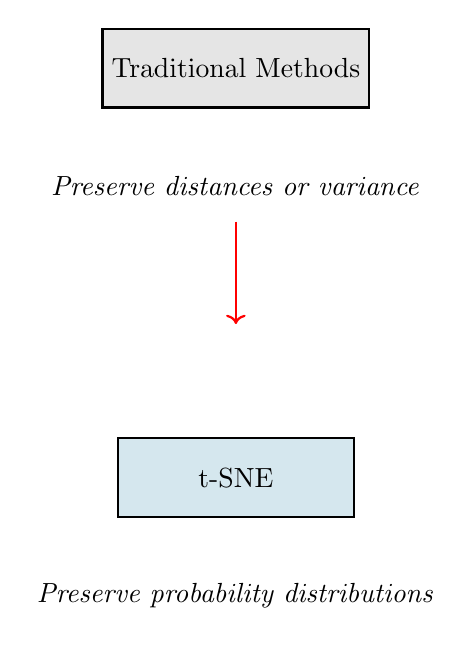
\begin{tikzpicture}[scale=1.3]
\node[draw, thick, fill=gray!20, minimum width=3cm, minimum height=1cm] (trad) at (0,3) {Traditional Methods};
\node[below of=trad, yshift=-0.5cm] {\textit{Preserve distances or variance}};
\draw[thick, red, ->] (0,1.5) -- (0,0.5);

\node[draw, thick, fill=highDcolor!20, minimum width=3cm, minimum height=1cm] (tsne) at (0,-1) {t-SNE};
\node[below of=tsne, yshift=-0.5cm] {\textit{Preserve probability distributions}};
\end{tikzpicture}
\end{center}

\vspace{0.3cm}
\begin{block}{Key Insight}
Instead of asking "How close are points?" we ask "How likely are they neighbors?"
\end{block}
\end{frame}


% Slide 5b - IMPROVED AESTHETIC VERSION
\begin{frame}{The Paradigm Shift: Concrete Example}
\begin{columns}
\column{0.5\textwidth}
\begin{tcolorbox}[colback=blue!5, colframe=blue!40, title={\textbf{Traditional: Preserve Distances}}]
\begin{center}
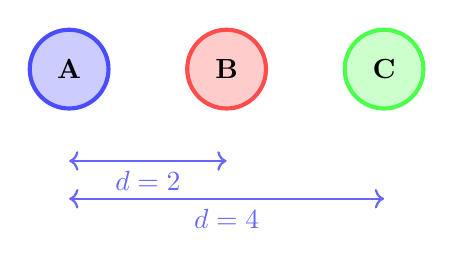
\begin{tikzpicture}[scale=0.8]
% Three points with better styling
\node[circle, draw=blue!70, fill=blue!20, line width=1.5pt, minimum size=10mm] (A) at (0,0) {\textbf{A}};
\node[circle, draw=red!70, fill=red!20, line width=1.5pt, minimum size=10mm] (B) at (2.5,0) {\textbf{B}};
\node[circle, draw=green!70, fill=green!20, line width=1.5pt, minimum size=10mm] (C) at (5,0) {\textbf{C}};

% Distance arcs
\draw[<->, thick, blue!60] ([yshift=-8mm]A.south) -- ([yshift=-8mm]B.south) node[midway, below] {$d=2$};
\draw[<->, thick, blue!60] ([yshift=-14mm]A.south) -- ([yshift=-14mm]C.south) node[midway, below] {$d=4$};
\end{tikzpicture}
\end{center}
\vspace{3mm}
\textcolor{red!70}{Problem:} All distances treated equally\\
\textcolor{gray}{No context about local density}
\end{tcolorbox}

\column{0.5\textwidth}
\begin{tcolorbox}[colback=green!5, colframe=green!40, title={\textbf{t-SNE: Preserve Probabilities}}]
\begin{center}
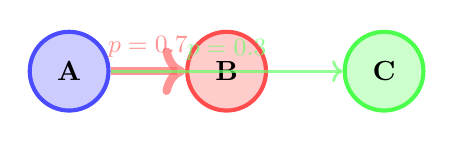
\begin{tikzpicture}[scale=0.8]
% Three points with probability visualization
\node[circle, draw=blue!70, fill=blue!20, line width=1.5pt, minimum size=10mm] (A) at (0,0) {\textbf{A}};
\node[circle, draw=red!70, fill=red!20, line width=1.5pt, minimum size=10mm] (B) at (2.5,0) {\textbf{B}};
\node[circle, draw=green!70, fill=green!20, line width=1.5pt, minimum size=10mm] (C) at (5,0) {\textbf{C}};

% Probability arrows with varying thickness
\draw[->, line width=3pt, red!60, opacity=0.7] (A) -- (B) node[midway, above] {\small $p=0.7$};
\draw[->, line width=1pt, green!60, opacity=0.7] (A) -- (C) node[midway, above] {\small $p=0.3$};
\end{tikzpicture}
\end{center}
\vspace{3mm}
\textcolor{green!70}{Solution:} Likelihood encodes context\\
\textcolor{gray}{Adapts to local density automatically}
\end{tcolorbox}
\end{columns}

\vspace{0.5cm}
\begin{tcolorbox}[colback=yellow!10, colframe=orange!60, boxrule=1pt]
\centering
\textbf{Key Insight:} Same distance $\rightarrow$ different probabilities based on neighborhood density
\end{tcolorbox}
\end{frame}

% ADD THIS AFTER SLIDE 5 (The Paradigm Shift)
\begin{frame}{Why Probability Distributions for Neighborhoods?}
\textbf{The Fundamental Question:}\\
How do we mathematically represent "neighborliness" between points?

\begin{columns}
\column{0.5\textwidth}
\textbf{Option 1: Binary (Yes/No)}
\begin{itemize}
\item Neighbor or not neighbor
\item Problem: Too rigid!
\item Loses gradual relationships
\end{itemize}

\textbf{Option 2: Raw Distances}
\begin{itemize}
\item Use actual measurements
\item Problem: No context!
\item 5 units means different things
\end{itemize}

\column{0.5\textwidth}
\textbf{Option 3: Probabilities ✓}
\begin{itemize}
\item Continuous values [0,1]
\item Context-aware (adapts to density)
\item Mathematically tractable
\item Information theory foundation
\end{itemize}

\begin{center}
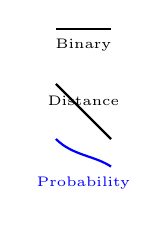
\begin{tikzpicture}[scale=0.7]
% Binary
\draw[thick] (0,2) -- (1,2);
\node at (0.5,1.7) {\tiny Binary};
% Distance
\draw[thick] (0,1) -- (1,0);
\node at (0.5,0.7) {\tiny Distance};
% Probability
\draw[thick, blue] (0,0) .. controls (0.3,-0.3) and (0.7,-0.3) .. (1,-0.5);
\node at (0.5,-0.8) {\tiny \textcolor{blue}{Probability}};
\end{tikzpicture}
\end{center}
\end{columns}

\vspace{0.3cm}
\colorbox{green!20}{Next: How to convert distances to probabilities mathematically}
\end{frame}

\begin{frame}{Building Intuition: From Distances to Neighborhoods}
\begin{columns}
\column{0.5\textwidth}
\textbf{The Problem with Raw Distances:}
\begin{itemize}
\item Point A: 1 unit from B, 10 units from C
\item But what if A is in dense region?
\item And C is in sparse region?
\item Raw distance loses context!
\end{itemize}

\vspace{0.3cm}
\textbf{The Solution - Relative Similarity:}
\begin{itemize}
\item Convert distances to probabilities
\item "How likely is B to be A's neighbor?"
\item Adapt to local density automatically
\item Use Gaussian decay (smooth, differentiable)
\end{itemize}

\column{0.5\textwidth}
\begin{center}
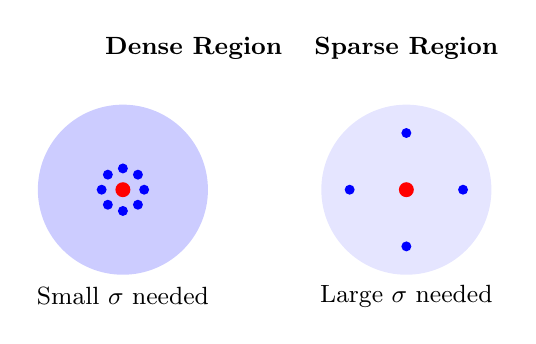
\begin{tikzpicture}[scale=0.9]
% Dense region example
\node at (0,2) {\small\textbf{Dense Region}};
\fill[blue!20] (-1,0) circle (1.2);
\fill[red] (-1,0) circle (3pt);
\foreach \angle in {0,45,...,315} {
    \fill[blue] (-1,0) ++(\angle:0.3) circle (2pt);
}
\node at (-1,-1.5) {\small Small $\sigma$ needed};

% Sparse region example  
\node at (3,2) {\small\textbf{Sparse Region}};
\fill[blue!10] (3,0) circle (1.2);
\fill[red] (3,0) circle (3pt);
\foreach \angle in {0,90,180,270} {
    \fill[blue] (3,0) ++(\angle:0.8) circle (2pt);
}
\node at (3,-1.5) {\small Large $\sigma$ needed};
\end{tikzpicture}
\end{center}

\vspace{0.2cm}
\textbf{Key Idea:} Each point gets its own "neighborhood size" ($\sigma_i$) based on local density
\end{columns}
\end{frame}

% Slide 5
\begin{frame}{From Distances to Probabilities}
\begin{columns}
\column{0.5\textwidth}
\begin{center}
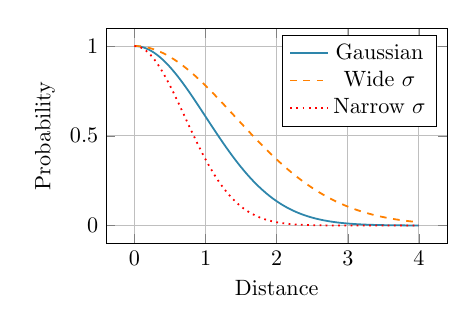
\begin{tikzpicture}[scale=0.8]
\begin{axis}[
    xlabel={Distance},
    ylabel={Probability},
    width=7cm,
    height=5cm,
    grid=major,
    legend pos=north east
]
\addplot[domain=0:4, samples=100, thick, highDcolor] {exp(-x^2/2)};
\addlegendentry{Gaussian}
\addplot[domain=0:4, samples=100, thick, orange, dashed] {exp(-x^2/4)};
\addlegendentry{Wide $\sigma$}
\addplot[domain=0:4, samples=100, thick, red, dotted] {exp(-x^2/1)};
\addlegendentry{Narrow $\sigma$}
\end{axis}
\end{tikzpicture}
\end{center}

\column{0.5\textwidth}
\textbf{Key Transformation:}
$$p_{j|i} = \frac{\exp(-\|x_i - x_j\|^2/2\sigma_i^2)}{\sum_{k \neq i} \exp(-\|x_i - x_k\|^2/2\sigma_i^2)}$$

\vspace{0.3cm}
\insight{$\sigma_i$ adapts to local density automatically}
\end{columns}
\end{frame}


% Slide 6a - INTUITIVE VERSION
\begin{frame}{Why Gaussian? The Natural Choice for Neighborhoods}
\begin{columns}
\column{0.5\textwidth}
\begin{tcolorbox}[colback=blue!5, colframe=blue!40, title={\textbf{What We're Building}}]
\textbf{Our Goal:}
\begin{itemize}
\item Convert distances to probabilities
\item "How likely is j to be i's neighbor?"
\item Must adapt to local density
\end{itemize}

\vspace{3mm}
\textbf{Three Key Requirements:}
\begin{enumerate}
\item \textcolor{blue}{Smooth decay} - no sudden cutoffs
\item \textcolor{green}{Local focus} - neighbors matter most
\item \textcolor{red}{Unbiased} - don't assume patterns
\end{enumerate}

\vspace{3mm}
\textbf{The Winner: Gaussian}
\vspace{-2mm}
$p_{j|i} \propto e^{-d_{ij}^2/2\sigma_i^2}$
\end{tcolorbox}

\column{0.5\textwidth}
\begin{center}
\textbf{Visual Comparison}\\[3mm]
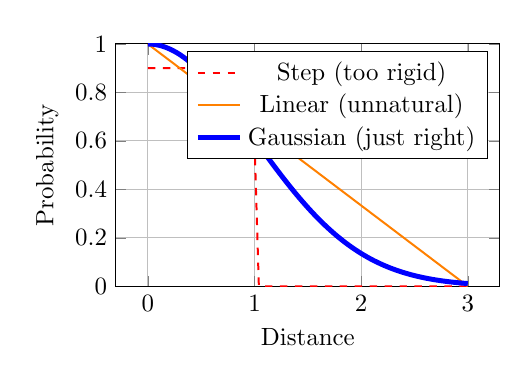
\begin{tikzpicture}[scale=0.9]
\begin{axis}[
    width=7cm,
    height=5cm,
    xlabel={Distance},
    ylabel={Probability},
    legend pos=north east,
    grid=major,
    ymin=0, ymax=1
]
% Step function - too rigid
\addplot[domain=0:3, samples=50, thick, red, dashed] {0.9*(x<1)};
\addlegendentry{Step (too rigid)}

% Linear - unnatural
\addplot[domain=0:3, samples=50, thick, orange] {max(0, 1-x/3)};
\addlegendentry{Linear (unnatural)}

% Gaussian - just right
\addplot[domain=0:3, samples=100, thick, blue, line width=2pt] {exp(-x^2/2)};
\addlegendentry{Gaussian (just right)}
\end{axis}
\end{tikzpicture}
\end{center}

\vspace{3mm}
\begin{tcolorbox}[colback=green!5, colframe=green!40, boxrule=0.5pt]
\centering\small
\textbf{Analogy:} Friendship strength\\
strongest nearby, fading smoothly
\end{tcolorbox}
\end{columns}
\end{frame}

% Slide 6b - MATHEMATICAL PRINCIPLE
\begin{frame}{The Mathematics Behind Gaussian: Maximum Entropy Principle}
\begin{columns}
\column{0.55\textwidth}
\begin{tcolorbox}[colback=yellow!5, colframe=orange!40, title={\textbf{The Core Principle}}]
\textbf{The Question:}\\
Which distribution makes the \textit{fewest assumptions} while matching our constraints?

\vspace{4mm}
\textbf{Answer: Maximum Entropy}\\
The distribution with highest uncertainty (entropy) given the constraints

\vspace{4mm}
\textbf{Why This Matters:}
\begin{itemize}
\item Most "honest" - no hidden bias
\item Adds no assumptions
\item Principled approach
\end{itemize}
\end{tcolorbox}

\column{0.45\textwidth}
\begin{center}
\textbf{Entropy Comparison}\\[3mm]
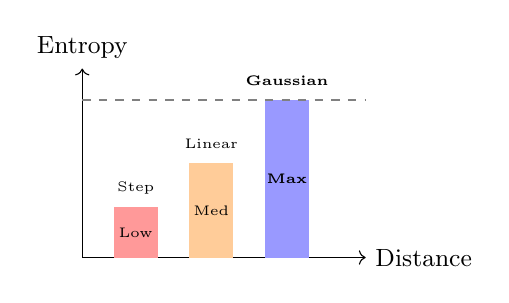
\begin{tikzpicture}[scale=0.8]
\draw[->] (0,0) -- (4.5,0) node[right] {\small Distance};
\draw[->] (0,0) -- (0,3) node[above] {\small Entropy};

% Bars showing entropy levels
\fill[red!40] (0.5,0) rectangle (1.2,0.8);
\node at (0.85,1.1) {\tiny Step};
\node at (0.85,0.4) {\tiny Low};

\fill[orange!40] (1.7,0) rectangle (2.4,1.5);
\node at (2.05,1.8) {\tiny Linear};
\node at (2.05,0.75) {\tiny Med};

\fill[blue!40] (2.9,0) rectangle (3.6,2.5);
\node at (3.25,2.8) {\tiny \textbf{Gaussian}};
\node at (3.25,1.25) {\tiny \textbf{Max}};

\draw[dashed, gray] (0,2.5) -- (4.5,2.5);
\end{tikzpicture}
\end{center}

\vspace{3mm}
\begin{tcolorbox}[colback=blue!5, colframe=blue!40]
\centering\small
\textbf{Gaussian = Maximum Entropy}\\
Most uncertain = Least biased
\end{tcolorbox}
\end{columns}
\end{frame}

% --- SLIDE 1: The Optimization Problem ---
\begin{frame}{The Mathematical Derivation: Problem Setup}
    \begin{tcolorbox}[colback=yellow!5, colframe=orange!40, title={\textbf{Optimization Problem}}]
    \textbf{Maximize Entropy:}
    \[H(P_i) = -\sum_j p_{j|i} \log p_{j|i}\]

    \textbf{Subject to Constraints:}
    \begin{enumerate}
    \item Normalization: $\sum_j p_{j|i} = 1$
    \item Fixed Variance: $\sum_j p_{j|i} d_{ij}^2 = \sigma_i^2$
    \end{enumerate}
    
    \vspace{2mm}
    \textit{The goal is to find the most unbiased probability distribution ($p_{j|i}$) that meets our constraints.}
    \end{tcolorbox}
\end{frame}


% --- SLIDE 2: The Solution ---
\begin{frame}{The Mathematical Derivation: Solution}
    \begin{tcolorbox}[colback=blue!5, colframe=blue!40, title={\textbf{Solution via Lagrange Multipliers}}]
    
    \textbf{1. The Lagrangian:}
    \begin{align*}
    \mathcal{L} = H(P_i) &+ \lambda \left(\sum p_{j|i} - 1\right) \\
                         &+ \mu \left(\sum p_{j|i}d_{ij}^2 - \sigma_i^2\right)
    \end{align*}
    
    \vspace{1mm}
    \textbf{2. Taking derivatives and solving for $\frac{\partial \mathcal{L}}{\partial p_{j|i}} = 0$ yields the result.}
    \vspace{1mm}
    
    \textbf{3. Result (The Gaussian Distribution):}
    \[
    p_{j|i} = \frac{e^{-\frac{d_{ij}^2}{2\sigma_i^2}}}{\sum_k e^{-\frac{d_{ik}^2}{2\sigma_i^2}}}
    \]
    
    \end{tcolorbox}
\end{frame}


% Slide 7 - REVISED VERSION
\begin{frame}{Perplexity: Setting the Neighborhood Size}
\begin{columns}
\column{0.5\textwidth}
\begin{tcolorbox}[colback=blue!5, colframe=blue!40, title={\textbf{The Problem We're Solving}}]
\textbf{Question:} How many neighbors should each point consider?

\vspace{3mm}
\textbf{Challenge:} Different regions have different densities!
\begin{itemize}
\item Dense areas: Small $\sigma$ needed
\item Sparse areas: Large $\sigma$ needed
\end{itemize}

\vspace{3mm}
\textbf{Solution:} Perplexity - a user parameter that sets "effective" number of neighbors
\end{tcolorbox}

\column{0.5\textwidth}
\begin{center}
\textbf{Adaptive Neighborhoods}\\[3mm]
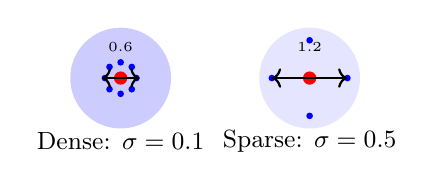
\begin{tikzpicture}[scale=0.8]
% Dense region
\fill[blue!20] (-1,1) circle (0.8);
\fill[red] (-1,1) circle (3pt);
\foreach \angle in {0,45,...,315} {
    \fill[blue] (-1,1) ++(\angle:0.25) circle (1.5pt);
}
\node at (-1,0) {\small Dense: $\sigma = 0.1$};
\draw[<->, thick] (-1.3,1) -- (-0.7,1);
\node at (-1,1.5) {\tiny 0.6};

% Sparse region  
\fill[blue!10] (2,1) circle (0.8);
\fill[red] (2,1) circle (3pt);
\foreach \angle in {0,90,180,270} {
    \fill[blue] (2,1) ++(\angle:0.6) circle (1.5pt);
}
\node at (2,0) {\small Sparse: $\sigma = 0.5$};
\draw[<->, thick] (1.4,1) -- (2.6,1);
\node at (2,1.5) {\tiny 1.2};
\end{tikzpicture}

\vspace{3mm}
\begin{tcolorbox}[colback=green!5, colframe=green!40]
\centering\small
Both have same perplexity = 5\\
Different $\sigma$ values!
\end{tcolorbox}
\end{center}
\end{columns}

\vspace{1mm}
\begin{tcolorbox}[colback=yellow!10, colframe=orange!60]
\centering
\textbf{Key Insight:} Perplexity is constant across all points, but $\sigma_i$ adapts to achieve it
\end{tcolorbox}
\end{frame}

% Slide 7b - MATHEMATICAL DEFINITION AND BINARY SEARCH
\begin{frame}{Perplexity: The Mathematics and Algorithm}
\begin{columns}
\column{0.5\textwidth}
\begin{tcolorbox}[colback=blue!5, colframe=blue!40, title={\textbf{Mathematical Definition}}]
\textbf{From Shannon Entropy:}
$$H(P_i) = -\sum_j p_{j|i} \log_2 p_{j|i}$$

\vspace{2mm}
\textbf{Perplexity:}
$$\text{Perp}(P_i) = 2^{H(P_i)}$$

\vspace{1mm}
\textbf{Interpretation:}
\begin{itemize}
\item Perp = 5 → "acts like" 5 neighbors
\item Perp = 30 → "acts like" 30 neighbors
\item Typical range: 5-50
\end{itemize}

\small\textit{Note: It's the exponential of entropy!}
\end{tcolorbox}

\column{0.5\textwidth}
\begin{tcolorbox}[colback=orange!5, colframe=orange!40, title={\textbf{Finding $\sigma_i$: Binary Search}}]
\small
\textbf{Why Binary Search?}\\
Perplexity increases with $\sigma$ monotonically

\vspace{2mm}
\begin{center}
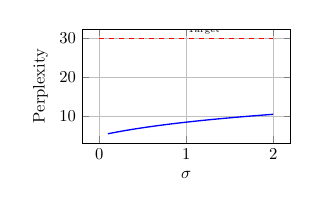
\begin{tikzpicture}[scale=0.6]
\begin{axis}[
    width=6cm,
    height=4cm,
    xlabel={$\sigma$},
    ylabel={Perplexity},
    grid=major
]
\addplot[domain=0.1:2, samples=50, thick, blue] {5*ln(x+1)+5};
\addplot[dashed, red] coordinates {(0,30) (2,30)};
\node at (axis cs:1.2,32) {\tiny Target};
\end{axis}
\end{tikzpicture}
\end{center}

\textbf{Algorithm:}
\begin{enumerate}
\item Start with $\sigma = 1$
\item Compute current perplexity
\item Too high? → Decrease $\sigma$
\item Too low? → Increase $\sigma$
\item Repeat until converged
\end{enumerate}
\normalsize
\end{tcolorbox}
\end{columns}
\end{frame}


% Slide 8 - REVISED VERSION
\begin{frame}{Measuring Information Loss: KL Divergence}
\vspace{-3mm}
\begin{columns}
\column{0.55\textwidth}
\begin{block}{What is KL Divergence?}
$$\text{KL}(P||Q) = \sum_j p_j \log\frac{p_j}{q_j}$$
\small
\textit{Extra bits needed when using $Q$ instead of true $P$}
\end{block}

\vspace{2mm}
\begin{block}{Critical Asymmetry Example}
\small
Consider point B with true probability 0.3:\\[2mm]
\textcolor{red}{\textbf{Missing a true neighbor:}}\\
True: $p = 0.3$, Embedded: $q = 0.01$\\
Penalty: $0.3 \times \log(30) \approx \textbf{1.02 bits}$\\[2mm]

\textcolor{blue}{\textbf{Creating a false neighbor:}}\\
True: $p = 0.01$, Embedded: $q = 0.3$\\
Penalty: $0.01 \times \log(0.033) \approx \textbf{-0.035 bits}$
\end{block}

\column{0.45\textwidth}
\begin{center}
\textbf{Visual Example}\\[2mm]
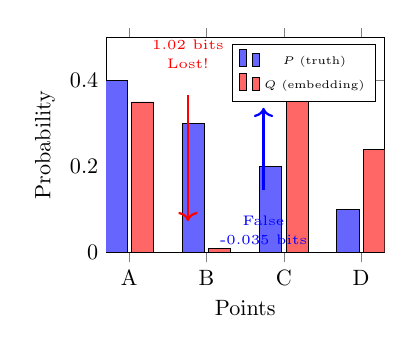
\begin{tikzpicture}[scale=0.8]
\begin{axis}[
  ybar,
  width=6cm,
  height=5cm,
  ylabel={Probability},
  xlabel={Points},
  symbolic x coords={A,B,C,D},
  xtick=data,
  ymin=0, ymax=0.5,
  legend pos=north east,
  legend style={font=\tiny}
]
\addplot[fill=blue!60] coordinates {(A,0.4) (B,0.3) (C,0.2) (D,0.1)};
\addplot[fill=red!60] coordinates {(A,0.35) (B,0.01) (C,0.4) (D,0.24)};
\legend{$P$ (truth), $Q$ (embedding)}
\end{axis}

% Annotations showing penalties
\draw[->, thick, red] (1.3, 2.5) -- (1.3, 0.5);
\node[red] at (1.3, 3) {\tiny Lost!};
\node[red] at (1.3, 3.3) {\tiny 1.02 bits};

\draw[->, thick, blue] (2.5, 1) -- (2.5, 2.3);
\node[blue] at (2.5, 0.5) {\tiny False};
\node[blue] at (2.5, 0.2) {\tiny -0.035 bits};
\end{tikzpicture}
\end{center}
\end{columns}

\vspace{2mm}
\begin{center}
\colorbox{yellow!20}{\parbox{0.9\textwidth}{\centering
\textbf{Key Insight:} t-SNE heavily penalizes separating true neighbors (30× more than false neighbors!)}}
\end{center}
\end{frame}



% Slide 9a - CONCEPTUAL INTRODUCTION
\begin{frame}{Original SNE: The Precursor to t-SNE}
\begin{center}
\textbf{A Brief History of Dimension Reduction}
\end{center}

\vspace{5mm}
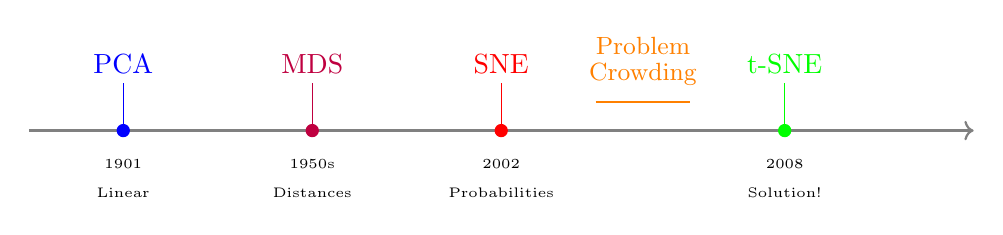
\begin{tikzpicture}[scale=1.2]
% Timeline
\draw[thick, ->, gray] (0,0) -- (10,0);

% PCA
\fill[blue] (1,0) circle (2pt);
\draw[blue] (1,0) -- (1,0.5);
\node[above, blue] at (1,0.5) {PCA};
\node[below] at (1,-0.2) {\tiny 1901};
\node[below] at (1,-0.5) {\tiny Linear};

% MDS
\fill[purple] (3,0) circle (2pt);
\draw[purple] (3,0) -- (3,0.5);
\node[above, purple] at (3,0.5) {MDS};
\node[below] at (3,-0.2) {\tiny 1950s};
\node[below] at (3,-0.5) {\tiny Distances};

% SNE
\fill[red] (5,0) circle (2pt);
\draw[red] (5,0) -- (5,0.5);
\node[above, red] at (5,0.5) {SNE};
\node[below] at (5,-0.2) {\tiny 2002};
\node[below] at (5,-0.5) {\tiny Probabilities};

% Problem
\draw[orange, thick] (6,0.3) -- (7,0.3);
\node[orange] at (6.5,0.6) {\small Crowding};
\node[orange] at (6.5,0.9) {\small Problem};

% t-SNE
\fill[green] (8,0) circle (2pt);
\draw[green] (8,0) -- (8,0.5);
\node[above, green] at (8,0.5) {t-SNE};
\node[below] at (8,-0.2) {\tiny 2008};
\node[below] at (8,-0.5) {\tiny Solution!};
\end{tikzpicture}

\vspace{8mm}
\begin{columns}
\column{0.5\textwidth}
\begin{block}{SNE's Innovation}
\begin{itemize}
\item First to use probabilities
\item Adaptive neighborhoods ($\sigma_i$)
\item Information-theoretic approach
\item KL divergence for optimization
\end{itemize}
\end{block}

\column{0.5\textwidth}
\begin{block}{SNE's Fatal Flaw}
\begin{itemize}
\item Used Gaussian in low-D space
\item Cannot represent moderate distances
\item Led to "crowding problem"
\item All points collapse together
\end{itemize}
\end{block}
\end{columns}

\vspace{1mm}
\begin{center}
\colorbox{yellow!20}{\parbox{0.9\textwidth}{\centering
\textbf{Key Lesson:} Great ideas can fail on one crucial detail}}
\end{center}
\end{frame}


\begin{frame}{SNE's Mathematics: Where It Went Wrong}
% --- 2. Use [T] to top-align the columns ---
\begin{columns}[T]

    % --- Left Column: The Formulation ---
    \column{0.5\textwidth}
\begin{block}{The Formulation}
    \begin{itemize}
        \item \textbf{High-D Similarity ($P$):} \\
              Gaussian with adaptive variance $\sigma_i$
              $$ p_{j|i} = \frac{\exp(-d_{ij}^2/2\sigma_i^2)}{\sum_k \exp(-d_{ik}^2/2\sigma_i^2)} $$

        \item \textbf{Low-D Similarity ($Q$):} \\
              \alert{Gaussian with fixed variance}
              $$ q_{j|i} = \frac{\exp(-d_{ij}^2)}{\sum_k \exp(-d_{ik}^2)} $$

        % CORRECTED LINE: The formula is now inline to save vertical space.
        \item \textbf{Cost Function:} $C = \sum_i \mathrm{KL}(P_i || Q_i)$
    \end{itemize}
\end{block}

% --- Right Column: The Problem in 2D ---
\column{0.5\textwidth}
\begin{block}{Why Gaussian Fails in 2D}
    \centering % Center the plot
    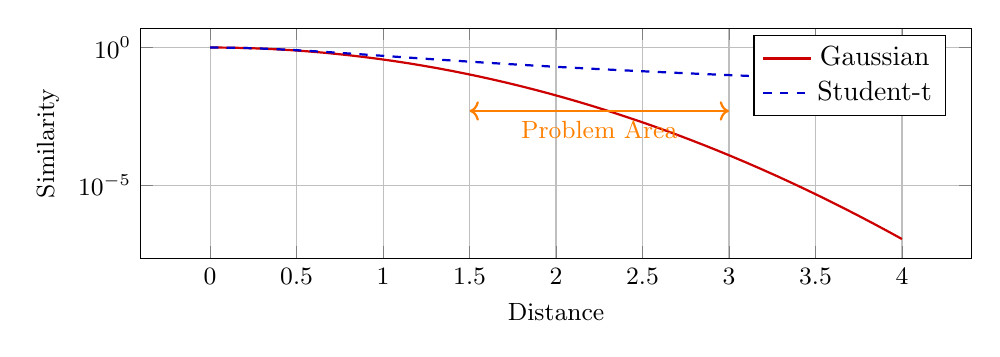
\begin{tikzpicture}
        \begin{axis}[
            width=\linewidth,
            height=4.5cm, % CORRECTED: Reduced height from 5cm
            xlabel={Distance},
            ylabel={Similarity},
            ymode=log,
            grid=major,
            legend pos=north east,
            label style={font=\small},
            tick label style={font=\small}
        ]
        \addplot[domain=0:4, samples=50, thick, red!80!black] {exp(-x^2)};
        \addlegendentry{Gaussian}
        
        \addplot[domain=0:4, samples=50, thick, blue!80!black, dashed] {1/(1+x^2)};
        \addlegendentry{Student-t}
        
        \draw[<->, orange, thick] (axis cs:1.5, 5e-3) -- (axis cs:3, 5e-3)
            node[midway, below, font=\small] {Problem Area};
        \end{axis}
    \end{tikzpicture}
    \small
    \alert{Problem:} Moderate distances in high-D get exponentially tiny similarities in low-D, causing crowding.
\end{block}

\end{columns}


\end{frame}

% Slide 10 - REVISED VERSION
\begin{frame}{The Curse: Why High-D Breaks Our Intuition}
\vspace{-3mm}
\begin{columns}
\column{0.5\textwidth}
\begin{block}{The Volume Problem}
\textbf{Question:} In a D-dimensional sphere,\\
what fraction of volume is in the outer\\
shell (radius 0.9 to 1.0)?

\vspace{3mm}
\textbf{Your intuition (2D):}
$$\frac{\pi \cdot 1^2 - \pi \cdot 0.9^2}{\pi \cdot 1^2} = 19\%$$

\textbf{Reality in high-D:}
\begin{itemize}
\item 5D: 41\%
\item 10D: 65\%
\item 50D: 99.5\%
\item \textcolor{red}{\textbf{100D: 99.997\%}}
\end{itemize}
\end{block}

\column{0.5\textwidth}
\begin{center}
\textbf{Volume Distribution by Dimension}\\[2mm]
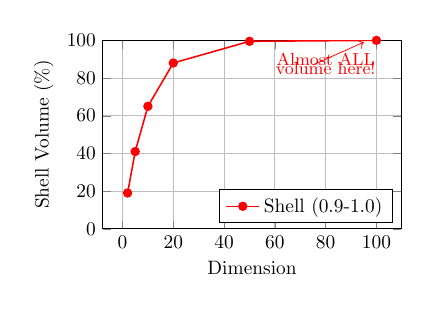
\begin{tikzpicture}[scale=0.7]
\begin{axis}[
  xlabel={Dimension},
  ylabel={Shell Volume (\%)},
  width=7cm,
  height=5cm,
  grid=major,
  ymin=0, ymax=100,
  legend pos=south east
]
\addplot[mark=*, thick, red, mark size=2pt] coordinates {
  (2,19) (5,41) (10,65) (20,88) (50,99.5) (100,99.997)
};
\addlegendentry{Shell (0.9-1.0)}

% Highlight the key point
\draw[red, very thick] (axis cs:100,99.997) circle (0.3);
\node[red] at (axis cs:80,90) {\small Almost ALL};
\node[red] at (axis cs:80,85) {\small volume here!};
\draw[red, ->] (axis cs:75,87) -- (axis cs:95,99);
\end{axis}
\end{tikzpicture}
\end{center}
\end{columns}

\vspace{3mm}
\begin{center}
\colorbox{orange!20}{\parbox{0.9\textwidth}{\centering
\textbf{Connection to SNE:} In high-D, all points are at similar distances (outer shell)\\
In 2D, we need room for varying distances that doesn't geometrically exist!}}
\end{center}
\end{frame}

% Slide 11
\begin{frame}{SNE's Fatal Flaw Visualized}
\begin{columns}
\column{0.5\textwidth}
\begin{center}
\textbf{High-D: Room for all}\\[0.3cm]
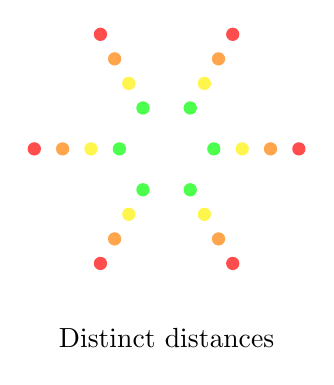
\begin{tikzpicture}[scale=1.2]
\foreach \r/\c in {0.5/green, 0.8/yellow, 1.1/orange, 1.4/red} {
    \foreach \a in {0,60,...,300} {
        \fill[\c!70] (\a:\r) circle (2pt);
    }
}
\node at (0,-2) {Distinct distances};
\end{tikzpicture}
\end{center}

\column{0.5\textwidth}
\begin{center}
\textbf{2D with Gaussian: Crushed!}\\[0.3cm]
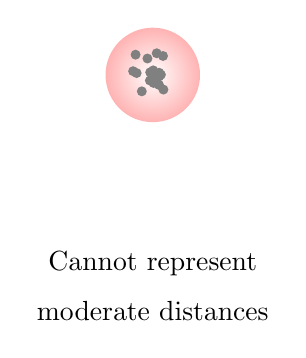
\begin{tikzpicture}[scale=1.2]
\shade[inner color=white, outer color=red!30] (0,0) circle (0.5);
\foreach \i in {1,...,20} {
    \pgfmathsetmacro\r{0.3*rnd}
    \pgfmathsetmacro\a{360*rnd}
    \fill[black!50] (\a:\r) circle (1.5pt);
}
\node at (0,-2) {Cannot represent};
\node at (0,-2.5) {moderate distances};
\end{tikzpicture}
\end{center}
\end{columns}

\vspace{0.3cm}
\begin{center}
\Large\textbf{Solution: Use distribution with heavier tails!}
\end{center}
\end{frame}


% Slide 12 - REVISED VERSION
\begin{frame}{The t-SNE Innovation: Student-t Distribution}
\vspace{-3mm}
\begin{columns}
\column{0.55\textwidth}
\begin{block}{The Key Change}
\textbf{SNE (Gaussian in 2D):}
$$q_{ij} = \frac{e^{-d_{ij}^2}}{\sum_{k \neq l} e^{-d_{kl}^2}}$$

\textbf{t-SNE (Student-t in 2D):}
$$q_{ij} = \frac{(1 + d_{ij}^2)^{-1}}{\sum_{k \neq l} (1 + d_{kl}^2)^{-1}}$$

\vspace{1mm}
\textbf{Mathematical Properties:}
\begin{itemize}
\item Polynomial decay: $O(d^{-2})$ vs exponential
\item Heavy tails preserve moderate distances
\item Cauchy distribution (df = 1)
\end{itemize}
\end{block}

\column{0.45\textwidth}
\begin{center}
\textbf{Decay Comparison}\\[2mm]
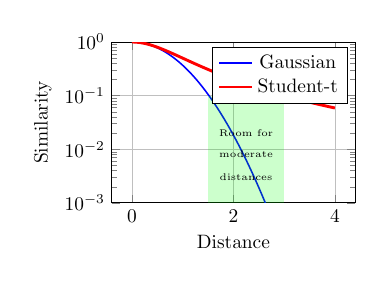
\begin{tikzpicture}[scale=0.7]
\begin{axis}[
    xlabel={Distance},
    ylabel={Similarity},
    width=6cm,
    height=4.5cm,
    grid=major,
    legend pos=north east,
    domain=0:4,
    ymode=log,
    ymin=0.001, ymax=1
]
\addplot[samples=100, thick, blue] {exp(-x^2)};
\addlegendentry{Gaussian}
\addplot[samples=100, thick, red, line width=1.5pt] {1/(1+x^2)};
\addlegendentry{Student-t}

% Mark the key difference region
\fill[green, opacity=0.2] (axis cs:1.5,0.001) rectangle (axis cs:3,0.1);
\node at (axis cs:2.25,0.02) {\tiny Room for};
\node at (axis cs:2.25,0.008) {\tiny moderate};
\node at (axis cs:2.25,0.003) {\tiny distances};
\end{axis}
\end{tikzpicture}
\end{center}
\end{columns}

\vspace{3mm}
\begin{center}
\colorbox{green!20}{\parbox{0.9\textwidth}{\centering
\textbf{How it solves crowding:} Heavy tails provide "space" for moderate distances\\
that doesn't exist geometrically in 2D but exists mathematically in the similarity function}}
\end{center}
\end{frame}

% Slide 13
\begin{frame}{Quantifying the Solution}
\begin{block}{Similarity Ratio Analysis}
For distances $d_1 = 1$ and $d_2 = 3$:
  \end{block}

\begin{columns}
\column{0.5\textwidth}
\textbf{Gaussian:}
$$\frac{q(d_1)}{q(d_2)} = \frac{e^{-1}}{e^{-9}} = e^8 \approx 2981$$
  \textcolor{red}{Moderate distance becomes "infinite"}

\column{0.5\textwidth}
\textbf{Student-t:}
$$\frac{q(d_1)}{q(d_2)} = \frac{1/(1+1)}{1/(1+9)} = 5$$
  \textcolor{green}{Moderate distance preserved}
\end{columns}

\vspace{0.5cm}
\begin{center}
\colorbox{yellow!30}{\Large 600× difference in representation capacity!}
\end{center}
\end{frame}


% Slide 14a - THE THREE KEY MODIFICATIONS
\begin{frame}{From SNE to t-SNE: Three Critical Changes}
\vspace{-3mm}
\begin{center}
\Large\textbf{The Evolution}
\end{center}

\vspace{1mm}
\begin{block}{Modification 1: Symmetrization}
\textbf{SNE:} Asymmetric $p_{j|i} \neq p_{i|j}$\\
\textbf{t-SNE:} Symmetric $p_{ij} = p_{ji} = \frac{p_{j|i} + p_{i|j}}{2n}$

\vspace{1mm}
\textbf{Why?} 
\begin{itemize}
\item Simplifies gradient (one term instead of two)
\item Ensures outliers get fair representation
\item More elegant optimization
\end{itemize}
\end{block}

\begin{block}{Modification 2: Student-t in Low-D}
\textbf{SNE:} $q_{ij} = \frac{\exp(-d_{ij}^2)}{\sum_{k \neq l}\exp(-d_{kl}^2)}$ (Gaussian)\\
\textbf{t-SNE:} $q_{ij} = \frac{(1+d_{ij}^2)^{-1}}{\sum_{k \neq l}(1+d_{kl}^2)^{-1}}$ (Student-t)

\vspace{1mm}
\textbf{Why?} Solves crowding with heavy tails
\end{block}

\begin{block}{Modification 3: Single KL Divergence}
\textbf{SNE:} $C = \sum_i \text{KL}(P_i||Q_i)$ (sum of individual KLs)\\
\textbf{t-SNE:} $C = \text{KL}(P||Q)$ (single joint KL)

\vspace{1mm}
\textbf{Why?} Works with symmetric probabilities
\end{block}
\end{frame}

% Slide 14b - THE UNIFIED ALGORITHM
\begin{frame}{The Complete t-SNE Algorithm}
\vspace{-3mm}
\begin{columns}
\column{0.5\textwidth}
\begin{block}{Input → Probabilities}
\textbf{1. Compute pairwise affinities:}
\small
$$p_{j|i} = \frac{\exp(-\|x_i-x_j\|^2/2\sigma_i^2)}{\sum_k \exp(-\|x_i-x_k\|^2/2\sigma_i^2)}$$
\normalsize

\textbf{2. Symmetrize:}
$$p_{ij} = \frac{p_{j|i} + p_{i|j}}{2n}$$

\textbf{3. Early exaggeration:}
$$p_{ij} \leftarrow 4 \cdot p_{ij} \text{ (first 250 iter)}$$
\end{block}

\column{0.5\textwidth}
\begin{block}{Optimization}
\textbf{4. Initialize:} $y_i \sim \mathcal{N}(0, 10^{-4})$

\textbf{5. Compute low-D similarities:}
\small
$$q_{ij} = \frac{(1+\|y_i-y_j\|^2)^{-1}}{\sum_{k \neq l}(1+\|y_k-y_l\|^2)^{-1}}$$
\normalsize

\textbf{6. Update via gradient:}
\small
$$\frac{\partial C}{\partial y_i} = 4\sum_j (p_{ij} - q_{ij})(y_i - y_j)(1 + d_{ij}^2)^{-1}$$
\normalsize

\textbf{7. Iterate until convergence}
\end{block}
\end{columns}

\vspace{3mm}
\begin{center}
\colorbox{blue!20}{\parbox{0.9\textwidth}{\centering
\textbf{Result:} An elegant algorithm that preserves local structure while solving crowding}}
\end{center}
\end{frame}

% Slide 15
\begin{frame}{Understanding the Gradient: Force Interpretation}
\begin{center}
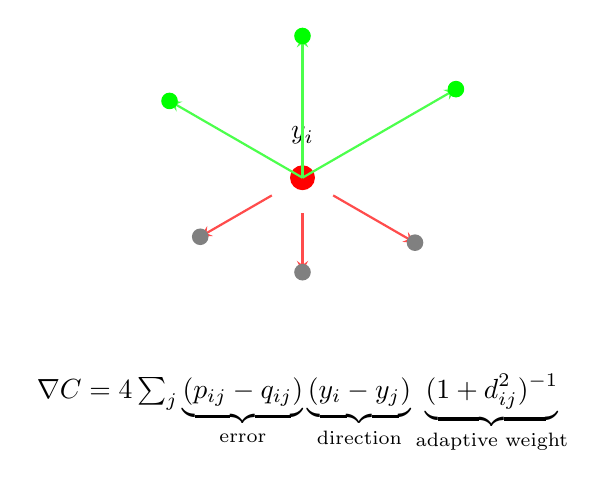
\begin{tikzpicture}[scale=1.5]
\fill[red] (0,0) circle (3pt);
\node[above] at (0,0.2) {$y_i$};

\foreach \angle/\dist in {30/1.5, 90/1.2, 150/1.3} {
  \draw[->, thick, green!70, >=stealth] (0,0) -- (\angle:\dist);
  \fill[green] (\angle:\dist) circle (2pt);
}

\foreach \angle/\dist in {210/1, 270/0.8, 330/1.1} {
  \draw[<-, thick, red!70, >=stealth] (\angle:\dist) -- (\angle:0.3);
  \fill[gray] (\angle:\dist) circle (2pt);
}

\node at (0,-2) {$\nabla C = 4\sum_j \underbrace{(p_{ij} - q_{ij})}_{\text{error}} \underbrace{(y_i - y_j)}_{\text{direction}} \underbrace{(1 + d_{ij}^2)^{-1}}_{\text{adaptive weight}}$};
\end{tikzpicture}
\end{center}

\insight{Weight term prevents distant clusters from merging}
\end{frame}


% Slide 16a - EARLY EXAGGERATION
\begin{frame}{Optimization Trick 1: Early Exaggeration}
\begin{columns}
\column{0.5\textwidth}
\begin{block}{The Technique}
\textbf{What:} Multiply $P$ by 4 for first 250 iterations
$$p_{ij}^{\text{early}} = 4 \cdot p_{ij}$$

\textbf{Effect on forces:}
\begin{itemize}
\item True neighbors pull 4× harder
\item Clusters form quickly
\item Global structure emerges first
\end{itemize}
\end{block}

\column{0.5\textwidth}
\begin{center}
\textbf{Visual Effect}\\[3mm]
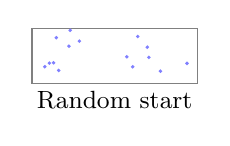
\begin{tikzpicture}[scale=0.7]
% Before
\draw[gray] (-1.5,-0.5) rectangle (1.5,0.5);
\foreach \i in {1,...,15} {
    \pgfmathsetmacro\x{3*rnd-1.5}
    \pgfmathsetmacro\y{rnd-0.5}
    \fill[blue!50] (\x,\y) circle (1pt);
}
\node at (0,-0.8) {\small Random start};
\end{tikzpicture}

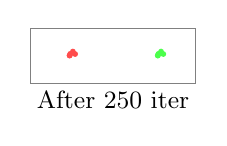
\begin{tikzpicture}[scale=0.7]
% After
\draw[gray] (-1.5,-0.5) rectangle (1.5,0.5);
\foreach \i in {1,...,5} {
    \pgfmathsetmacro\r{0.15*rnd}
    \pgfmathsetmacro\a{72*rnd}
    \fill[red!70] (-0.8,0) ++(\a:\r) circle (1.5pt);
    \fill[green!70] (0.8,0) ++(\a:\r) circle (1.5pt);
}
\node at (0,-0.8) {\small After 250 iter};
\end{tikzpicture}
\end{center}
\end{columns}

\vspace{3mm}
\begin{center}
\colorbox{green!20}{\parbox{0.85\textwidth}{\centering
Strong initial forces prevent poor local arrangements}}
\end{center}
\end{frame}

% Slide 16b - MOMENTUM
\begin{frame}{Optimization Trick 2: Momentum}
\begin{columns}
\column{0.5\textwidth}
\begin{block}{The Technique}
\textbf{Update equation:}
\small
$$\Delta y_i^{(t)} = -\eta \nabla_i + \alpha(t) \Delta y_i^{(t-1)}$$
\normalsize

\textbf{Schedule:}
$$\alpha(t) = \begin{cases}
0.5 & t < 250 \\
0.8 & t \geq 250
\end{cases}$$

\textbf{Benefits:}
\begin{itemize}
\item Escapes local minima
\item Smooths optimization
\item Reduces oscillations
\end{itemize}
\end{block}

\column{0.5\textwidth}
\begin{center}
\textbf{Effect on Optimization}\\[3mm]
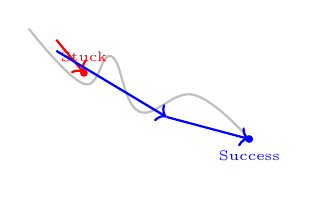
\begin{tikzpicture}[scale=0.7]
% Cost landscape
\draw[thick, gray!50] plot[smooth, tension=0.7] coordinates {(0,2) (1,1) (1.5,1.5) (2,0.5) (3,0.8) (4,0)};

% Without momentum
\draw[red, thick, ->] (0.5,1.8) -- (1,1.2);
\fill[red] (1,1.2) circle (2pt);
\node[red] at (1,1.5) {\tiny Stuck};

% With momentum
\draw[blue, thick, ->] (0.5,1.6) -- (2.5,0.4);
\draw[blue, thick, ->] (2.5,0.4) -- (4,0);
\fill[blue] (4,0) circle (2pt);
\node[blue] at (4,-0.3) {\tiny Success};
\end{tikzpicture}
\end{center}

\textbf{Analogy:} Ball rolling downhill - momentum carries it over bumps
\end{columns}
\end{frame}

% Slide 16c - ADAPTIVE LEARNING
\begin{frame}{Optimization Trick 3: Adaptive Learning Rate}
\begin{columns}
\column{0.5\textwidth}
\begin{block}{The Technique}
\textbf{Adaptation rule:}
\small
\begin{itemize}
\item Same direction: $\eta \times 1.2$
\item Direction change: $\eta \times 0.8$
\item Min: $\eta_{\min} = 0.01$
\item Max: $\eta_{\max} = 1000$
\end{itemize}
\normalsize

\textbf{Benefits:}
\begin{itemize}
\item Fast in flat regions
\item Careful near minima
\item Automatic adjustment
\end{itemize}
\end{block}

\column{0.5\textwidth}
\begin{center}
\textbf{Learning Rate Evolution}\\[3mm]
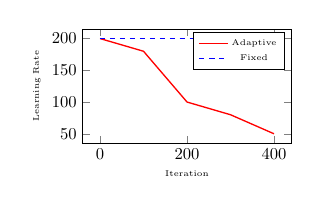
\begin{tikzpicture}[scale=0.6]
\begin{axis}[
    xlabel={\tiny Iteration},
    ylabel={\tiny Learning Rate},
    width=6cm,
    height=4cm,
    legend pos=north east,
    legend style={font=\tiny}
]
% Adaptive
\addplot[thick, red, mark=none] coordinates {
    (0,200) (100,180) (200,100) (300,80) (400,50)
};
\addlegendentry{Adaptive}

% Fixed
\addplot[thick, blue, dashed] coordinates {
    (0,200) (400,200)
};
\addlegendentry{Fixed}
\end{axis}
\end{tikzpicture}
\end{center}
\end{columns}

\vspace{3mm}
\begin{center}
\colorbox{green!20}{\parbox{0.85\textwidth}{\centering
\textbf{Combined:} 5× speedup (5000 → 1000 iterations)}}
\end{center}
\end{frame}


% Slide 17 - BARNES-HUT REVISED
\begin{frame}{Barnes-Hut: Scaling to Large Datasets}
\begin{columns}
\column{0.5\textwidth}
\begin{block}{The Algorithm}
\textbf{Key Idea:} Treat distant clusters as single points

\textbf{Steps:}
\begin{enumerate}
\item Build quadtree (2D) or octree (3D)
\item For each point, traverse tree
\item Apply criterion: $\frac{r_{\text{cell}}}{d_{\text{to cell}}} < \theta$
\item If satisfied, use center of mass
\end{enumerate}

\textbf{Parameter:} $\theta \in [0.5, 0.8]$\\
\small (higher = faster but less accurate)
\end{block}

\column{0.5\textwidth}
\begin{center}
\textbf{Tree Approximation}\\[2mm]
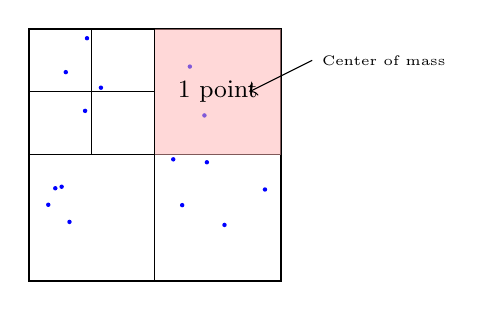
\begin{tikzpicture}[scale=0.8]
\draw[thick] (0,0) rectangle (4,4);
\draw (2,0) -- (2,4);
\draw (0,2) -- (4,2);
\draw (1,2) -- (1,4);
\draw (0,3) -- (2,3);

% Points
\foreach \i in {1,...,15} {
  \pgfmathsetmacro\x{4*rnd}
  \pgfmathsetmacro\y{4*rnd}
  \fill[blue] (\x,\y) circle (1pt);
}

% Highlight distant cell
\fill[red!30, opacity=0.5] (2,2) rectangle (4,4);
\node at (3,3) {\small 1 point};
\draw[<-] (3.5,3) -- (4.5,3.5) node[right] {\tiny Center of mass};
\end{tikzpicture}
\end{center}

\begin{center}
\begin{tabular}{l|r|r}
\textbf{Points} & \textbf{Exact} & \textbf{Barnes-Hut} \\
\hline
1,000 & 1 sec & 0.1 sec \\
10,000 & 100 sec & 2 sec \\
100,000 & 10,000 sec & 50 sec \\
\end{tabular}
\end{center}
\end{columns}
\end{frame}

% Slide 18 - DEBUGGING REVISED
\begin{frame}{Debugging t-SNE: Visual Diagnosis Guide}
\begin{center}
\textbf{Common Problems and Their Fixes}\\[3mm]
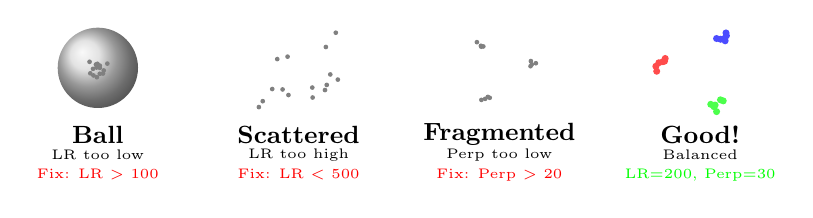
\begin{tikzpicture}[scale=0.85]
% Problem 1: Ball
\begin{scope}[shift={(0,0)}]
\shade[ball color=gray!30] (0,0) circle (0.6);
\foreach \i in {1,...,15} {
  \pgfmathsetmacro\r{0.2*rnd}
  \pgfmathsetmacro\a{24*\i}
  \fill[black!50] (\a:\r) circle (1pt);
}
\node at (0,-1) {\small\textbf{Ball}};
\node at (0,-1.3) {\tiny LR too low};
\node at (0,-1.6) {\tiny\textcolor{red}{Fix: LR > 100}};
\end{scope}

% Problem 2: Scattered
\begin{scope}[shift={(3,0)}]
\foreach \i in {1,...,15} {
  \pgfmathsetmacro\x{1.2*rnd-0.6}
  \pgfmathsetmacro\y{1.2*rnd-0.6}
  \fill[black!50] (\x,\y) circle (1pt);
}
\node at (0,-1) {\small\textbf{Scattered}};
\node at (0,-1.3) {\tiny LR too high};
\node at (0,-1.6) {\tiny\textcolor{red}{Fix: LR < 500}};
\end{scope}

% Problem 3: Fragmented
\begin{scope}[shift={(6,0)}]
\foreach \c in {0,120,240} {
  \foreach \i in {1,...,4} {
    \pgfmathsetmacro\r{0.15*rnd}
    \pgfmathsetmacro\a{\c+15*rnd}
    \fill[black!50] (\a:0.4+\r) circle (1pt);
  }
}
\node at (0,-1) {\small\textbf{Fragmented}};
\node at (0,-1.3) {\tiny Perp too low};
\node at (0,-1.6) {\tiny\textcolor{red}{Fix: Perp > 20}};
\end{scope}

% Problem 4: Good
\begin{scope}[shift={(9,0)}]
\foreach \c/\col in {45/blue,165/red,285/green} {
  \foreach \i in {1,...,6} {
    \pgfmathsetmacro\r{0.2*rnd}
    \pgfmathsetmacro\a{\c+20*rnd}
    \fill[\col!70] (\a:0.5+\r) circle (1.5pt);
  }
}
\node at (0,-1) {\small\textbf{Good!}};
\node at (0,-1.3) {\tiny Balanced};
\node at (0,-1.6) {\tiny\textcolor{green}{LR=200, Perp=30}};
\end{scope}
\end{tikzpicture}
\end{center}

\vspace{3mm}
\begin{center}
\colorbox{yellow!20}{\parbox{0.85\textwidth}{\centering
\textbf{Golden Rule:} Run multiple times with different seeds. Trust what's consistent.}}
\end{center}
\end{frame}

% Slide 19 - PERPLEXITY EFFECTS REVISED
\begin{frame}{Perplexity: Your Main Control Parameter}
\begin{columns}
\column{0.6\textwidth}
\begin{center}
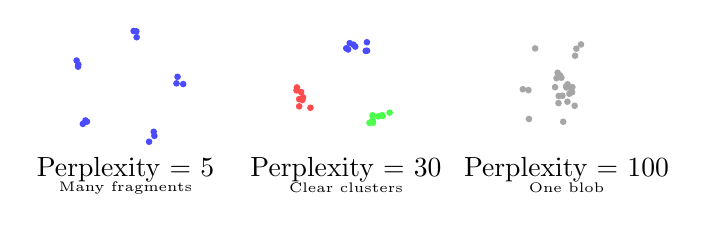
\begin{tikzpicture}[scale=0.8]
% Perp = 5
\begin{scope}[shift={(0,0)}]
\foreach \c in {0,72,144,216,288} {
  \foreach \i in {1,...,3} {
    \pgfmathsetmacro\r{0.15*rnd}
    \pgfmathsetmacro\a{\c+15*rnd}
    \fill[blue!70] (\a:0.8+\r) circle (1.5pt);
  }
}
\node at (0,-1.3) {Perplexity = 5};
\node at (0,-1.6) {\tiny Many fragments};
\end{scope}

% Perp = 30
\begin{scope}[shift={(3.5,0)}]
\foreach \c/\col in {60/blue,180/red,300/green} {
  \foreach \i in {1,...,8} {
    \pgfmathsetmacro\r{0.25*rnd}
    \pgfmathsetmacro\a{\c+30*rnd}
    \fill[\col!70] (\a:0.6+\r) circle (1.5pt);
  }
}
\node at (0,-1.3) {Perplexity = 30};
\node at (0,-1.6) {\tiny Clear clusters};
\end{scope}

% Perp = 100
\begin{scope}[shift={(7,0)}]
\foreach \i in {1,...,25} {
  \pgfmathsetmacro\r{0.8*rnd}
  \pgfmathsetmacro\a{360*rnd}
  \fill[gray!70] (\a:\r) circle (1.5pt);
}
\node at (0,-1.3) {Perplexity = 100};
\node at (0,-1.6) {\tiny One blob};
\end{scope}
\end{tikzpicture}
\end{center}

\column{0.4\textwidth}
\begin{block}{How to Choose?}
\textbf{Rule of thumb:}\\
Perp = $\sqrt{N}/10$ to $\sqrt{N}/2$\\
\small (N = number of points)

\vspace{3mm}
\textbf{Examples:}
\begin{itemize}
\item 1,000 points: 5-15
\item 10,000 points: 20-50
\item 100,000 points: 50-150
\end{itemize}

\vspace{3mm}
\textbf{Strategy:}
\begin{enumerate}
\item Try 3 values (low, mid, high)
\item Look for consistency
\item Trust stable structures
\end{enumerate}
\end{block}
\end{columns}

\vspace{3mm}
\begin{center}
\colorbox{blue!20}{\parbox{0.85\textwidth}{\centering
\textbf{Key Insight:} Truth is what's consistent across multiple perplexity values}}
\end{center}
\end{frame}

% Slide 20 - CRITICAL WARNINGS (MINIMAL CHANGES)
\begin{frame}{Critical: What You CANNOT Interpret}
\begin{center}
\Large\textcolor{red}{\textbf{The Three Deadly Sins of t-SNE}}
\end{center}

\vspace{3mm}
\begin{columns}
\column{0.33\textwidth}
\begin{center}
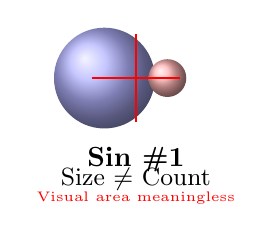
\begin{tikzpicture}[scale=0.8]
\shade[ball color=blue!30] (-0.5,0) circle (0.8);
\shade[ball color=red!30] (0.5,0) circle (0.3);
\draw[red, thick] (0,-0.7) -- (0,0.7);
\draw[red, thick] (-0.7,0) -- (0.7,0);
\node at (0,-1.3) {\textbf{Sin \#1}};
\node at (0,-1.6) {\small Size $\neq$ Count};
\node at (0,-1.9) {\tiny\textcolor{red}{Visual area meaningless}};
\end{tikzpicture}
\end{center}

\column{0.33\textwidth}
\begin{center}
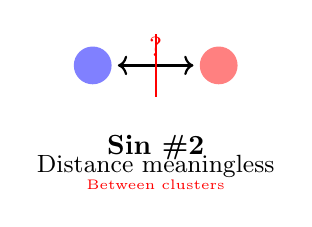
\begin{tikzpicture}[scale=0.8]
\fill[blue!50] (-1,0) circle (0.3);
\fill[red!50] (1,0) circle (0.3);
\draw[<->, thick] (-0.6,0) -- (0.6,0);
\node at (0,0.3) {\textcolor{red}{?}};
\draw[red, thick] (0,-0.5) -- (0,0.5);
\node at (0,-1.3) {\textbf{Sin \#2}};
\node at (0,-1.6) {\small Distance meaningless};
\node at (0,-1.9) {\tiny\textcolor{red}{Between clusters}};
\end{tikzpicture}
\end{center}

\column{0.33\textwidth}
\begin{center}
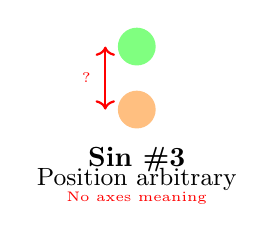
\begin{tikzpicture}[scale=0.8]
\fill[green!50] (0,0.5) circle (0.3);
\fill[orange!50] (0,-0.5) circle (0.3);
\draw[<->, red, thick] (-0.5,0.5) -- (-0.5,-0.5);
\node[red] at (-0.8,0) {\tiny ?};
\node at (0,-1.3) {\textbf{Sin \#3}};
\node at (0,-1.6) {\small Position arbitrary};
\node at (0,-1.9) {\tiny\textcolor{red}{No axes meaning}};
\end{tikzpicture}
\end{center}
\end{columns}

\vspace{5mm}
\begin{center}
\colorbox{yellow!20}{\parbox{0.85\textwidth}{\centering
\textbf{Remember:} Only local neighborhoods are meaningful. Everything else is artifact.}}
\end{center}
\end{frame}


% Slide 21 - MNIST CASE STUDY
\begin{frame}{MNIST Case Study: Complete Pipeline}
\begin{columns}
\column{0.5\textwidth}
\begin{block}{Data Preparation}
\textbf{1. Dataset:}
\begin{itemize}
\item 70,000 handwritten digits
\item 28×28 pixels = 784 dimensions
\end{itemize}

\textbf{2. Preprocessing:}
\begin{itemize}
\item Scale pixels to [0,1]
\item PCA to 50D (95\% variance)
\item Remove outliers $(>3\sigma)$
\end{itemize}

\textbf{3. t-SNE Settings:}
\begin{itemize}
\item Perplexity = 30
\item Learning rate = 200
\item Iterations = 1000
\end{itemize}
\end{block}

\column{0.5\textwidth}
\begin{center}
\textbf{Result: Clear Digit Separation}\\[3mm]
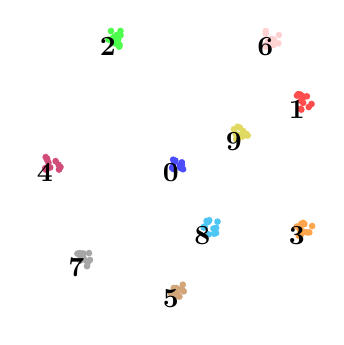
\begin{tikzpicture}[scale=0.8]
\foreach \d/\x/\y/\c in {
    0/0/0/blue,
    1/2/1/red,
    2/-1/2/green,
    3/2/-1/orange,
    4/-2/0/purple,
    5/0/-2/brown,
    6/1.5/2/pink,
    7/-1.5/-1.5/gray,
    8/0.5/-1/cyan,
    9/1/0.5/yellow!80!black} {
    \foreach \i in {1,...,12} {
        \pgfmathsetmacro\rx{0.25*rnd}
        \pgfmathsetmacro\ry{0.25*rnd}
        \fill[\c!70] (\x+\rx,\y+\ry) circle (1.5pt);
    }
    \node at (\x,\y) {\textbf{\d}};
}
\end{tikzpicture}

\vspace{3mm}
\textbf{Success indicators:}
\begin{itemize}
\item Each digit forms cluster
\item Similar digits nearby (7 near 1)
\item Clear boundaries
\end{itemize}
\end{center}
\end{columns}
\end{frame}

% Slide 22 - VALIDATION METRICS EXPLAINED
\begin{frame}{Quantitative Validation: Understanding the Metrics}
\begin{columns}
\column{0.5\textwidth}
\begin{block}{1. Neighborhood Preservation}
\textbf{What it measures:}\\
Do neighbors in high-D stay neighbors in 2D?

\textbf{Formula:}
$$\text{NPr}(k) = \frac{\text{overlap of } k \text{ neighbors}}{k}$$

\textbf{Good values:}
\begin{itemize}
\item NPr(10) $> 0.7$ ✓
\item NPr(30) $> 0.6$ ✓
\item NPr(50) $> 0.5$ ✓
\end{itemize}
\end{block}

\column{0.5\textwidth}
\begin{block}{2. Trustworthiness}
\textbf{What it measures:}\\
Are 2D neighbors actually close in high-D?

\textbf{Range:} 0 to 1 (higher = better)

\textbf{Good values:}
\begin{itemize}
\item T(10) $> 0.95$ ✓
\item T(30) $> 0.90$ ✓
\end{itemize}

\vspace{3mm}
\textbf{Continuity:} Similar but checks if high-D neighbors preserved
\end{block}
\end{columns}

\vspace{3mm}
\begin{center}
\colorbox{yellow!20}{\parbox{0.85\textwidth}{\centering
\textbf{Rule:} If NPr > 0.6 and T > 0.9, your embedding is trustworthy}}
\end{center}
\end{frame}

% Slide 23 - STABILITY ANALYSIS
\begin{frame}{Stability Analysis: Is Your Embedding Reliable?}
\begin{columns}
\column{0.5\textwidth}
\begin{block}{Testing Protocol}
\textbf{Steps:}
\begin{enumerate}
\item Run t-SNE 10 times
\item Different random seeds
\item Same parameters
\item Compare results
\end{enumerate}

\textbf{Measure correlation:}
\begin{itemize}
\item Between pairwise distances
\item Or cluster assignments
\end{itemize}
\end{block}

\column{0.5\textwidth}
\begin{center}
\textbf{Interpreting Results}\\[3mm]
\begin{tikzpicture}[scale=0.9]
% Good stability
\draw[green!20, fill=green!20] (0,0) rectangle (3,0.5);
\node[left] at (0,0.25) {$r > 0.9$};
\node[right] at (3,0.25) {\small Very stable ✓};

% Moderate
\draw[yellow!40, fill=yellow!40] (0,-0.7) rectangle (2.5,-.2);
\node[left] at (0,-0.45) {$r = 0.7-0.9$};
\node[right] at (2.5,-0.45) {\small Acceptable};

% Poor
\draw[red!20, fill=red!20] (0,-1.4) rectangle (2,-0.9);
\node[left] at (0,-1.15) {$r < 0.7$};
\node[right] at (2,-1.15) {\small Unreliable ✗};
\end{tikzpicture}

\vspace{5mm}
\textbf{Example correlation matrix:}\\
\small
\begin{tabular}{|c|c|c|c|}
\hline
Run & 1 & 2 & 3 \\
\hline
1 & 1.00 & 0.92 & 0.89 \\
2 & 0.92 & 1.00 & 0.91 \\
3 & 0.89 & 0.91 & 1.00 \\
\hline
\end{tabular}\\
\normalsize
Mean $r = 0.91$ → Very stable!
\end{center}
\end{columns}
\end{frame}

% Slide 24 - DATA PREPROCESSING
\begin{frame}{Critical: Data Preprocessing for t-SNE}
\begin{columns}
\column{0.5\textwidth}
\begin{block}{Essential Steps}
\textbf{1. Scaling (CRITICAL!)}
\begin{itemize}
\item Standardize: mean=0, std=1
\item Or normalize to [0,1]
\item \textcolor{red}{Never mix scales!}
\end{itemize}

\textbf{2. Dimensionality}
\begin{itemize}
\item If D > 50, use PCA first
\item Keep 95\% variance
\item Speeds computation 10×
\end{itemize}

\textbf{3. Missing Data}
\begin{itemize}
\item Impute with median
\item Or remove samples
\item Never use zeros!
\end{itemize}
\end{block}

\column{0.5\textwidth}
\begin{center}
\textbf{Preprocessing Pipeline}\\[3mm]
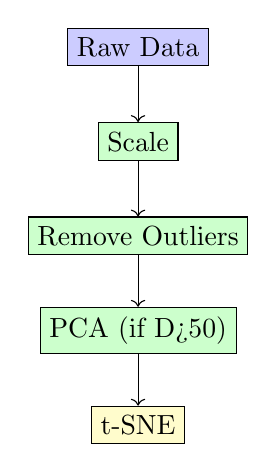
\begin{tikzpicture}[scale=0.8, node distance=1.5cm]
\node[draw, fill=blue!20] (raw) at (0,0) {Raw Data};
\node[draw, fill=green!20] (scale) at (0,-1.5) {Scale};
\node[draw, fill=green!20] (outlier) at (0,-3) {Remove Outliers};
\node[draw, fill=green!20] (pca) at (0,-4.5) {PCA (if D>50)};
\node[draw, fill=yellow!20] (tsne) at (0,-6) {t-SNE};

\draw[->] (raw) -- (scale);
\draw[->] (scale) -- (outlier);
\draw[->] (outlier) -- (pca);
\draw[->] (pca) -- (tsne);
\end{tikzpicture}
\end{center}

\vspace{3mm}
\begin{center}
\colorbox{red!20}{\parbox{0.8\textwidth}{\centering
Bad preprocessing = bad embedding,\\
regardless of t-SNE parameters!}}
\end{center}
\end{columns}
\end{frame}

% Slide 25 - t-SNE vs UMAP
\begin{frame}{Modern Alternatives: When to Use What}
\begin{center}
\begin{tabular}{l|c|c|c}
\textbf{Aspect} & \textbf{t-SNE} & \textbf{UMAP} & \textbf{Choose} \\
\hline
Speed & Slower & 5-10× faster & UMAP ✓ \\
Local structure & Excellent & Excellent & Tie \\
Global structure & Weak & Better & UMAP ✓ \\
Scalability & <100K & Millions & UMAP ✓ \\
Reproducibility & Random & More stable & UMAP ✓ \\
New points & No & Yes & UMAP ✓ \\
Interpretability & Intuitive & Complex & t-SNE ✓ \\
Fine detail & Better & Good & t-SNE ✓ \\
\end{tabular}
\end{center}

\vspace{5mm}
\begin{columns}
\column{0.5\textwidth}
\begin{center}
\colorbox{blue!20}{\parbox{0.9\textwidth}{\centering
\textbf{Use t-SNE when:}\\
\small
• Dataset < 50K points\\
• Local detail critical\\
• Publication figures\\
• Exploring clusters}}
\end{center}

\column{0.5\textwidth}
\begin{center}
\colorbox{green!20}{\parbox{0.9\textwidth}{\centering
\textbf{Use UMAP when:}\\
\small
• Large datasets\\
• Need speed\\
• Global structure matters\\
• Production systems}}
\end{center}
\end{columns}

\vspace{3mm}
\begin{center}
\colorbox{yellow!20}{\parbox{0.85\textwidth}{\centering
\textbf{Pro tip:} Use both and trust what's consistent between them}}
\end{center}
\end{frame}

% CONDENSED MATHEMATICAL ESSENTIALS (Replace slides 26-40 with these 5 slides)

% Slide 26 - WHY SYMMETRIZATION MATTERS
\begin{frame}{Mathematical Insight 1: Why Symmetrize?}
\begin{columns}
\column{0.5\textwidth}
\begin{block}{The Problem}
Original SNE uses asymmetric probabilities:
$$p_{j|i} \neq p_{i|j}$$

\textbf{Issue with outliers:}
\begin{itemize}
\item Outlier → others: very small
\item Others → outlier: normal
\item Result: Outliers disappear!
\end{itemize}
\end{block}

\column{0.5\textwidth}
\begin{block}{The Solution}
Symmetrization:
$$p_{ij} = \frac{p_{j|i} + p_{i|j}}{2n}$$

\begin{center}
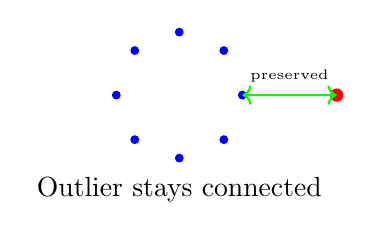
\begin{tikzpicture}[scale=0.8]
% Regular points
\foreach \i in {1,...,8} {
    \pgfmathsetmacro\a{45*\i}
    \fill[blue] (\a:1) circle (2pt);
}
% Outlier
\fill[red] (2.5,0) circle (3pt);
\draw[<->, thick, green] (1,0) -- (2.5,0);
\node at (1.75,0.3) {\tiny preserved};
\node at (0,-1.5) {Outlier stays connected};
\end{tikzpicture}
\end{center}
\end{block}
\end{columns}

\vspace{3mm}
\begin{center}
\colorbox{green!20}{\parbox{0.85\textwidth}{\centering
\textbf{Takeaway:} Symmetrization ensures every point gets fair representation}}
\end{center}
\end{frame}

% Slide 27 - THE GRADIENT SIMPLIFIED
\begin{frame}{Mathematical Insight 2: The Elegant Gradient}
\begin{center}
\Large The t-SNE gradient has beautiful structure:\\[5mm]
\normalsize
$$\frac{\partial C}{\partial y_i} = 4\sum_j \underbrace{(p_{ij} - q_{ij})}_{\text{error}} \cdot \underbrace{(y_i - y_j)}_{\text{direction}} \cdot \underbrace{(1 + d_{ij}^2)^{-1}}_{\text{adaptive weight}}$$
\end{center}

\vspace{5mm}
\begin{columns}
\column{0.33\textwidth}
\begin{center}
\textbf{Error Term}\\
$(p_{ij} - q_{ij})$\\[3mm]
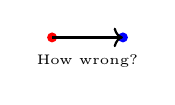
\begin{tikzpicture}[scale=0.6]
\fill[red] (0,0) circle (3pt);
\fill[blue] (1.5,0) circle (3pt);
\draw[thick, ->] (0,0) -- (1.5,0);
\node at (0.75,-0.5) {\tiny How wrong?};
\end{tikzpicture}
\end{center}

\column{0.33\textwidth}
\begin{center}
\textbf{Direction}\\
$(y_i - y_j)$\\[3mm]
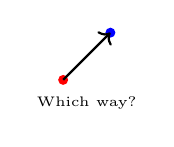
\begin{tikzpicture}[scale=0.6]
\fill[red] (0,0) circle (3pt);
\fill[blue] (1,1) circle (3pt);
\draw[thick, ->] (0,0) -- (1,1);
\node at (0.5,-0.5) {\tiny Which way?};
\end{tikzpicture}
\end{center}

\column{0.33\textwidth}
\begin{center}
\textbf{Adaptive Weight}\\
$(1 + d_{ij}^2)^{-1}$\\[3mm]
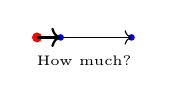
\begin{tikzpicture}[scale=0.6]
\fill[red] (0,0) circle (3pt);
\fill[blue] (0.5,0) circle (2pt);
\fill[blue] (2,0) circle (2pt);
\draw[thick, ->] (0,0) -- (0.5,0);
\draw[thin, ->] (0,0) -- (2,0);
\node at (1,-0.5) {\tiny How much?};
\end{tikzpicture}
\end{center}
\end{columns}

\vspace{5mm}
\begin{center}
\colorbox{blue!20}{\parbox{0.85\textwidth}{\centering
\textbf{Beautiful:} Nearby points get strong forces, distant points get weak forces}}
\end{center}
\end{frame}

% Slide 28 - WHY STUDENT-T WITH DF=1
\begin{frame}{Mathematical Insight 3: Why Exactly df=1?}
\begin{columns}
\column{0.5\textwidth}
\begin{block}{The Student-t Family}
General form with df=$\nu$:
$$q_{ij} \propto (1 + d_{ij}^2/\nu)^{-(\nu+1)/2}$$

\textbf{Special case $\nu=1$:}
$$q_{ij} \propto (1 + d_{ij}^2)^{-1}$$

This is the Cauchy distribution!
\end{block}

\vspace{1mm}
\begin{block}{Why df=1 is Perfect}
\begin{itemize}
\item Heaviest possible tails
\item Simplest gradient formula
\item Maximum space for moderate distances
\end{itemize}
\end{block}

\column{0.5\textwidth}
\begin{center}
\textbf{Tail Thickness Comparison}\\[3mm]
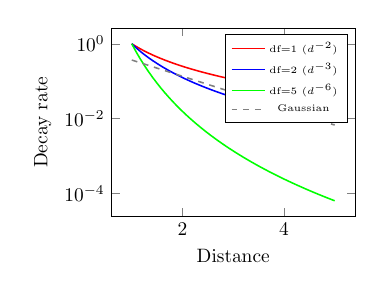
\begin{tikzpicture}[scale=0.7]
\begin{axis}[
    xlabel={Distance},
    ylabel={Decay rate},
    width=6cm,
    height=5cm,
    ymode=log,
    legend pos=north east,
    legend style={font=\tiny}
]
\addplot[domain=1:5, samples=50, thick, red] {x^(-2)};
\addlegendentry{df=1 ($d^{-2}$)}

\addplot[domain=1:5, samples=50, thick, blue] {x^(-3)};
\addlegendentry{df=2 ($d^{-3}$)}

\addplot[domain=1:5, samples=50, thick, green] {x^(-6)};
\addlegendentry{df=5 ($d^{-6}$)}

\addplot[domain=1:5, samples=50, thick, gray, dashed] {exp(-x)};
\addlegendentry{Gaussian}
\end{axis}
\end{tikzpicture}

\vspace{3mm}
df=1 has the slowest decay\\
= most room for moderate distances
\end{center}
\end{columns}
\end{frame}

% Slide 29 - COMPUTATIONAL COMPLEXITY
\begin{frame}{Practical Math: Computational Complexity}
\begin{center}
\begin{tabular}{l|c|c|c}
\textbf{Algorithm} & \textbf{Time} & \textbf{Space} & \textbf{Practical Limit} \\
\hline
\hline
Exact t-SNE & $O(n^2)$ & $O(n^2)$ & 5,000 points \\
Barnes-Hut & $O(n \log n)$ & $O(n)$ & 100,000 points \\
FFT-accelerated & $O(n)$ & $O(n)$ & 10 million points \\
\hline
\end{tabular}
\end{center}

\vspace{5mm}
\begin{columns}
\column{0.5\textwidth}
\begin{block}{Where Time Goes}
\begin{itemize}
\item Computing $P$: Once, $O(n^2)$
\item Computing $Q$: Every iteration
\item Gradient: Every iteration
\item Total: $\sim 1000$ iterations
\end{itemize}
\end{block}

\column{0.5\textwidth}
\begin{block}{Speed Tips}
\begin{itemize}
\item PCA to 50D first: 10× speedup
\item Barnes-Hut: 50× speedup
\item Fewer iterations: 2× speedup
\item GPU: 10-200× speedup
\end{itemize}
\end{block}
\end{columns}

\vspace{3mm}
\begin{center}
\colorbox{yellow!20}{\parbox{0.85\textwidth}{\centering
\textbf{Rule of thumb:} 10K points = 1 minute, 100K points = 1 hour (CPU)}}
\end{center}
\end{frame}

% Slide 30 - WHEN MATH MATTERS
\begin{frame}{When Does the Math Actually Matter?}
\begin{columns}
\column{0.5\textwidth}
\begin{block}{Math You Can Ignore}
\textcolor{gray}{For most users:}
\begin{itemize}
\item Lagrangian derivations
\item Exact gradient formulas
\item Entropy calculations
\item Proof details
\end{itemize}

\vspace{3mm}
Just use the default implementation!
\end{block}

\column{0.5\textwidth}
\begin{block}{Math You Should Know}
\textcolor{blue}{For better results:}
\begin{itemize}
\item Perplexity $\sim$ expected neighbors
\item Heavy tails prevent crowding
\item Local vs global structure trade-off
\item Why preprocessing matters
\end{itemize}

\vspace{3mm}
This helps you debug problems!
\end{block}
\end{columns}

\vspace{5mm}
\begin{center}
\colorbox{green!20}{\parbox{0.85\textwidth}{\centering
\textbf{The 80/20 Rule:}\\
Understanding 20\% of the math gives you 80\% of the practical benefit}}
\end{center}
\end{frame}


% Slide 41 - SINGLE-CELL GENOMICS APPLICATION
\begin{frame}{Real-World Impact: Single-Cell Genomics}
\begin{columns}
\column{0.5\textwidth}
\begin{block}{The Challenge}
\textbf{Data characteristics:}
\begin{itemize}
\item 20,000+ genes per cell
\item 100,000+ cells per experiment
\item 90\%+ zeros (sparse data)
\item Batch effects between samples
\end{itemize}

\textbf{Processing pipeline:}
\begin{enumerate}
\item Log-normalize counts
\item Select top 2000 variable genes
\item PCA to 50 components
\item t-SNE with perplexity 30-100
\end{enumerate}

\textbf{Computational requirements:}
\begin{itemize}
\item Time: 2-4 hours (100K cells)
\item RAM: 32-64 GB
\item Software: Seurat, Scanpy
\end{itemize}
\end{block}

\column{0.5\textwidth}
\begin{center}
\textbf{Discovering Cell Types}\\[3mm]
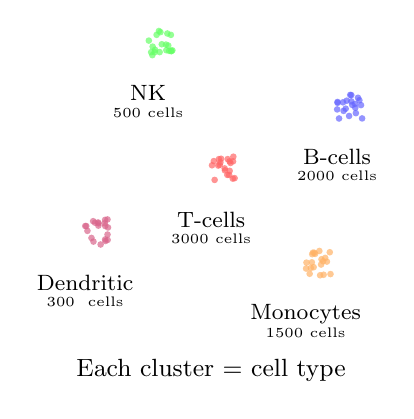
\begin{tikzpicture}[scale=0.8]
% Cell type clusters with labels
\foreach \type/\x/\y/\col/\name/\count in {
    1/0/0/red/T-cells/3000,
    2/2/1/blue/B-cells/2000,
    3/-1/2/green/NK/500,
    4/1.5/-1.5/orange/Monocytes/1500,
    5/-2/-1/purple/Dendritic/300
} {
    \foreach \i in {1,...,20} {
        \pgfmathsetmacro\rx{0.4*rnd}
        \pgfmathsetmacro\ry{0.4*rnd}
        \fill[\col!60, opacity=0.7] (\x+\rx,\y+\ry) circle (1.5pt);
    }
    \node at (\x,\y-0.6) {\footnotesize\name};
    \node at (\x,\y-0.9) {\tiny\count\ cells};
}
\node at (0,-3) {\small Each cluster = cell type};
\end{tikzpicture}
\end{center}

\textbf{Impact:} Found 3 new cell subtypes in 2019 leading to new cancer therapies
\end{columns}
\end{frame}

% Slide 42 - NLP APPLICATION
\begin{frame}{NLP Revolution: Word Embeddings Visualization}
\begin{columns}
\column{0.5\textwidth}
\begin{block}{The Pipeline}
\textbf{Data preparation:}
\begin{itemize}
\item Word2Vec/BERT embeddings
\item 300-768 dimensions
\item Vocabulary: 10K-50K words
\item Cosine distance metric
\end{itemize}

\textbf{t-SNE parameters:}
\begin{itemize}
\item Perplexity: 20-50
\item Learning rate: 500
\item Iterations: 5000
\item Metric: cosine (not Euclidean!)
\end{itemize}

\textbf{Computational cost:}
\begin{itemize}
\item 10K words: 5 minutes
\item 50K words: 45 minutes
\item GPU recommended for >20K
\end{itemize}
\end{block}

\column{0.5\textwidth}
\begin{center}
\textbf{Semantic Clusters Revealed}\\[3mm]
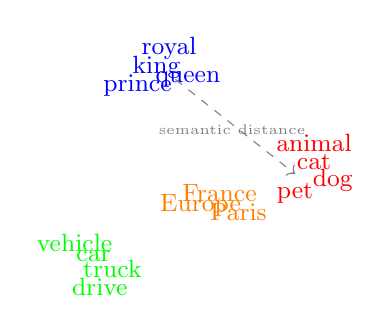
\begin{tikzpicture}[scale=0.8]
% Royal cluster
\node[blue] at (0,2) {\small king};
\node[blue] at (0.5,1.8) {\small queen};
\node[blue] at (-0.3,1.7) {\small prince};
\node[blue] at (0.2,2.3) {\small royal};

% Animal cluster
\node[red] at (2.5,0.5) {\small cat};
\node[red] at (2.8,0.2) {\small dog};
\node[red] at (2.2,0) {\small pet};
\node[red] at (2.5,0.8) {\small animal};

% Vehicle cluster
\node[green] at (-1,-1) {\small car};
\node[green] at (-0.7,-1.2) {\small truck};
\node[green] at (-1.3,-0.8) {\small vehicle};
\node[green] at (-0.9,-1.5) {\small drive};

% Country cluster
\node[orange] at (1,0) {\small France};
\node[orange] at (1.3,-0.3) {\small Paris};
\node[orange] at (0.7,-0.2) {\small Europe};

% Show relationships
\draw[->, gray, dashed] (0.3,1.8) -- (2.2,0.3);
\node[gray] at (1.2,1) {\tiny semantic distance};
\end{tikzpicture}
\end{center}

\textbf{Key insight:} Analogies preserved!\\
king - man + woman $\sim$ queen
\end{columns}
\end{frame}

% Slide 43 - DEEP LEARNING APPLICATION
\begin{frame}{Deep Learning: Understanding Neural Networks}
\begin{columns}
\column{0.5\textwidth}
\begin{block}{Visualizing CNN Features}
\textbf{What to visualize:}
\begin{itemize}
\item Layer activations (conv5, fc7)
\item 512-4096 dimensional vectors
\item Per image or per class
\end{itemize}

\textbf{Implementation:}
\footnotesize
\begin{enumerate}
\item Extract features: 1 min/1K images
\item PCA to 50D: 10 seconds
\item t-SNE: 5-15 minutes
\item Total: <20 min for 10K images
\end{enumerate}
\normalsize

\textbf{Hardware requirements:}
\begin{itemize}
\item GPU for feature extraction
\item 16GB RAM minimum
\end{itemize}
\end{block}

\column{0.5\textwidth}
\begin{center}
\textbf{What You Discover}\\[3mm]
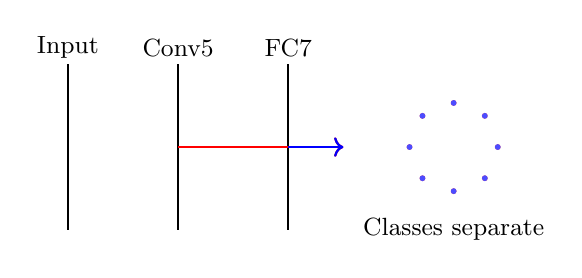
\begin{tikzpicture}[scale=0.7]
% Network diagram
\draw[thick] (0,0) -- (0,3);
\draw[thick] (2,0) -- (2,3);
\draw[thick] (4,0) -- (4,3);

\node at (0,3.3) {\small Input};
\node at (2,3.3) {\small Conv5};
\node at (4,3.3) {\small FC7};

% Arrows to t-SNE
\draw[->, thick, red] (2,1.5) -- (5,1.5);
\draw[->, thick, blue] (4,1.5) -- (5,1.5);

% t-SNE result
\begin{scope}[shift={(7,1.5)}]
\foreach \i in {1,...,8} {
    \pgfmathsetmacro\a{45*\i}
    \pgfmathsetmacro\r{0.8}
    \fill[red!70] (\a:\r) circle (1.5pt);
}
\foreach \i in {1,...,8} {
    \pgfmathsetmacro\a{45*\i+180}
    \pgfmathsetmacro\r{0.8}
    \fill[blue!70] (\a:\r) circle (1.5pt);
}
\node at (0,-1.5) {\small Classes separate};
\end{scope}
\end{tikzpicture}
\end{center}

\textbf{Discoveries made:}
\begin{itemize}
\item Hierarchy emerges (dogs near wolves)
\item Confusion patterns visible
\item Dead neurons identified
\item Adversarial vulnerabilities found
\end{itemize}
\end{columns}
\end{frame}


% ADVANCED METHODS - CONDENSED FROM 17 TO 5 SLIDES

% Slide 44 - OVERVIEW OF EXTENSIONS
\begin{frame}{Beyond Basic t-SNE: Advanced Methods Overview}
\begin{center}
\textbf{Choose Your Enhancement Based on Your Need}
\end{center}

\vspace{3mm}
\begin{tabular}{l|l|l}
\textbf{Your Problem} & \textbf{Solution} & \textbf{Trade-off} \\
\hline
Need to embed new data & Parametric t-SNE & 10× slower training \\
Data changes over time & Dynamic t-SNE & Complex parameters \\
Dataset > 100K points & GPU acceleration & Requires CUDA \\
Need inverse mapping & Parametric t-SNE & Less flexible \\
Multiple scales important & Multi-scale t-SNE & More parameters \\
Want global structure & UMAP instead & Different algorithm \\
\end{tabular}

\vspace{5mm}
\begin{center}
\colorbox{yellow!20}{\parbox{0.85\textwidth}{\centering
\textbf{Reality check:} 90\% of users just need standard t-SNE with good parameters}}
\end{center}
\end{frame}

% Slide 45 - PARAMETRIC T-SNE
\begin{frame}{Parametric t-SNE: Learning a Mapping Function}
\begin{columns}
\column{0.5\textwidth}
\begin{block}{How It Works}
Instead of just finding positions, learn a function $f_\theta: \mathbb{R}^d \to \mathbb{R}^2$

\textbf{Architecture:}
\begin{itemize}
\item Neural network (3-5 layers)
\item Input: high-D data
\item Output: 2D coordinates
\item Train to minimize t-SNE loss
\end{itemize}

\textbf{When to use:}
\begin{itemize}
\item Streaming data
\item Need to embed new points
\item Production systems
\end{itemize}
\end{block}

\column{0.5\textwidth}
\begin{block}{Practical Details}
\textbf{Advantages:}
\begin{itemize}
\item Embed new data instantly
\item Consistent mapping
\item Can learn inverse
\end{itemize}

\textbf{Disadvantages:}
\begin{itemize}
\item 10× slower to train
\item Slightly worse quality
\item Needs more tuning
\end{itemize}

\textbf{Implementation:}
\begin{itemize}
\item Library: \texttt{parametric\_tsne}
\item Time: 2-5 hours for 50K points
\item GPU recommended
\end{itemize}
\end{block}
\end{columns}
\end{frame}

% Slide 46 - GPU ACCELERATION
\begin{frame}[fragile]{GPU Acceleration: Scaling to Millions}
\begin{columns}
\column{0.5\textwidth}
\begin{block}{Performance Gains}
\begin{center}
\begin{tabular}{l|r|r}
\textbf{Dataset} & \textbf{CPU} & \textbf{GPU} \\
\hline
10K & 2 min & 10 sec \\
100K & 2 hours & 5 min \\
1M & Days & 1 hour \\
\end{tabular}
\end{center}

\vspace{3mm}
\textbf{Speedup:} 20-200× typical
\end{block}

\vspace{3mm}
\begin{block}{Requirements}
\begin{itemize}
\item NVIDIA GPU ($\geq$ 4GB VRAM)
\item CUDA toolkit installed
\item Libraries: RAPIDS, cuda-tsne
\end{itemize}
\end{block}

\column{0.5\textwidth}
\begin{block}{Implementation Tips}
\textbf{Best practices:}
\begin{itemize}
\item Batch size = 512-1024
\item Use mixed precision
\item Monitor GPU memory
\end{itemize}

\textbf{Code example:}
\footnotesize
\begin{verbatim}
# RAPIDS cuML
from cuml import TSNE
tsne = TSNE(n_components=2,
            perplexity=30,
            method='fft')  # Fast!
Y = tsne.fit_transform(X)
\end{verbatim}
\normalsize

\textbf{Cloud options:}
\begin{itemize}
\item Google Colab (free tier)
\item AWS EC2 p3 instances
\item \$1-3/hour typical cost
\end{itemize}
\end{block}
\end{columns}
\end{frame}

% Slide 47 - DYNAMIC T-SNE
\begin{frame}{Dynamic t-SNE: Visualizing Change Over Time}
\begin{columns}
\column{0.5\textwidth}
\begin{block}{The Approach}
Add temporal coherence to cost:
$$C_{\text{total}} = C_{\text{t-SNE}} + \lambda C_{\text{temporal}}$$

\textbf{Use cases:}
\begin{itemize}
\item Gene expression over time
\item Topic evolution in text
\item Learning progression
\item Market dynamics
\end{itemize}

\textbf{Key parameter:}\\
$\lambda$ = stability vs accuracy\\
\small (0.1-0.5 typical)
\end{block}

\column{0.5\textwidth}
\begin{center}
\textbf{Visualization Example}\\[3mm]
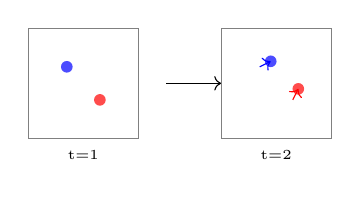
\begin{tikzpicture}[scale=0.7]
% Time 1
\begin{scope}[shift={(0,0)}]
\draw[gray] (-1,-1) rectangle (1,1);
\fill[blue!70] (-0.3,0.3) circle (3pt);
\fill[red!70] (0.3,-0.3) circle (3pt);
\node at (0,-1.3) {\tiny t=1};
\end{scope}

% Arrow
\draw[->] (1.5,0) -- (2.5,0);

% Time 2
\begin{scope}[shift={(3.5,0)}]
\draw[gray] (-1,-1) rectangle (1,1);
\fill[blue!70] (-0.1,0.4) circle (3pt);
\fill[red!70] (0.4,-0.1) circle (3pt);
\draw[blue, ->] (-0.3,0.3) -- (-0.1,0.4);
\draw[red, ->] (0.3,-0.3) -- (0.4,-0.1);
\node at (0,-1.3) {\tiny t=2};
\end{scope}
\end{tikzpicture}

Points move smoothly between frames
\end{center}

\textbf{Implementation:}
\begin{itemize}
\item Process all timepoints together
\item 2-3× slower than static
\item Results: animated visualization
\end{itemize}
\end{columns}
\end{frame}

% Slide 48 - PRACTICAL DECISION TREE
\begin{frame}{Which Method Should You Actually Use?}
\begin{center}
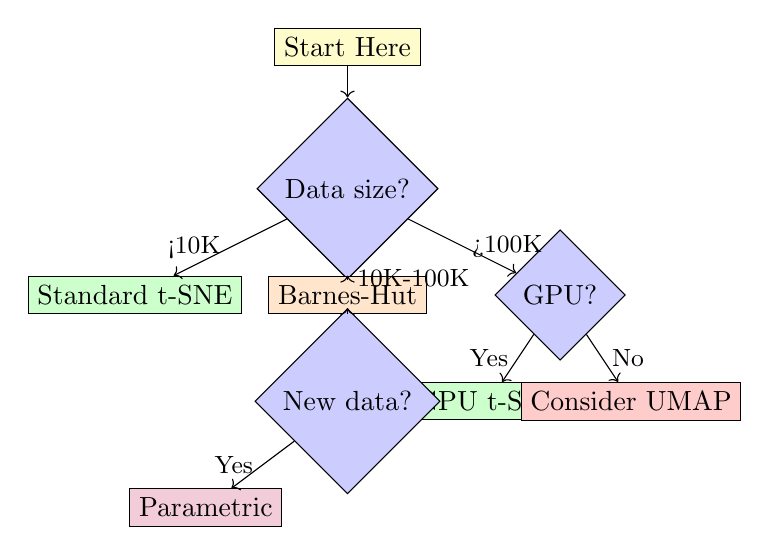
\begin{tikzpicture}[scale=0.9, node distance=2cm]
% Start
\node[draw, fill=yellow!20] (start) at (0,0) {Start Here};

% First decision
\node[draw, diamond, fill=blue!20] (size) at (0,-2) {Data size?};
\draw[->] (start) -- (size);

% Size branches
\node[draw, fill=green!20] (small) at (-3,-3.5) {Standard t-SNE};
\draw[->] (size) -- node[left] {\small <10K} (small);

\node[draw, fill=orange!20] (medium) at (0,-3.5) {Barnes-Hut};
\draw[->] (size) -- node[right] {\small 10K-100K} (medium);

\node[draw, diamond, fill=blue!20] (gpu) at (3,-3.5) {GPU?};
\draw[->] (size) -- node[right] {\small >100K} (gpu);

% GPU branches
\node[draw, fill=green!20] (yesgpu) at (2,-5) {GPU t-SNE};
\draw[->] (gpu) -- node[left] {\small Yes} (yesgpu);

\node[draw, fill=red!20] (nogpu) at (4,-5) {Consider UMAP};
\draw[->] (gpu) -- node[right] {\small No} (nogpu);

% New data branch
\node[draw, diamond, fill=blue!20] (newdata) at (0,-5) {New data?};
\draw[->] (medium) -- (newdata);

\node[draw, fill=purple!20] (param) at (-2,-6.5) {Parametric};
\draw[->] (newdata) -- node[left] {\small Yes} (param);
\end{tikzpicture}
\end{center}

\vspace{3mm}
\begin{center}
\colorbox{green!20}{\parbox{0.85\textwidth}{\centering
\textbf{Default recipe:} Barnes-Hut t-SNE, perplexity=30, iterations=1000}}
\end{center}
\end{frame}

% REPLACE SLIDES 61-75 WITH THESE 3 SLIDES

% New Slide 61 (Replaces old 61-63)
\begin{frame}{Key Extensions for Specialized Cases}
\textbf{When Standard t-SNE Isn't Enough:}

\begin{columns}
\column{0.55\textwidth}
\textbf{Supervised t-SNE (Fisher Kernel):}
\begin{itemize}
\item Incorporates class labels
\item Modifies: $p_{ij} \times (1+\lambda)$ if same class
\item Better class separation
\item Use when: Labels available
\end{itemize}

\textbf{Alternative Kernels:}
\begin{itemize}
\item $\alpha$-SNE: $(1 + d^2)^{-\alpha}$ 
\item Controls tail heaviness
\item Use for specific distance needs
\end{itemize}

\column{0.45\textwidth}
\small
\begin{tabular}{l|l|l}
\textbf{Method} & \textbf{Best For} & \textbf{Cost} \\
\hline
Standard & Exploration & $O(n \log n)$ \\
Fisher & Classification & $O(n \log n)$ \\
$\alpha$-SNE & Custom & $O(n^2)$ \\
Parametric & New data & $O(n)$ + train \\
\end{tabular}

\vspace{0.3cm}
\insight{Most users need only standard t-SNE. Consider extensions for specific requirements.}
\end{columns}
\end{frame}

% New Slide 62 (Replaces old 64-70)
\begin{frame}{Scaling to Millions of Points}
\textbf{Three Approaches for Large-Scale t-SNE:}

\begin{columns}
\column{0.6\textwidth}
\textbf{1. Approximation Methods:}
\begin{itemize}
\item \textbf{Random Walk:} Sample neighborhoods stochastically
\item \textbf{Landmarks:} Embed subset, interpolate others
\item \textbf{FFT:} For $d \leq 3$, use grid interpolation
\end{itemize}

\textbf{2. Computational Optimizations:}
\begin{itemize}
\item \textbf{GPU:} 50-100x speedup (RAPIDS, cuda-tsne)
\item \textbf{Distributed:} Split across machines
\item \textbf{Progressive:} Start with subset, add points
\end{itemize}

\textbf{3. Out-of-Sample Extension:}
\begin{itemize}
\item Train on subset, project new points
\item Use parametric t-SNE or kernel regression
\end{itemize}

\column{0.4\textwidth}
\begin{center}
\textbf{Decision Tree:}
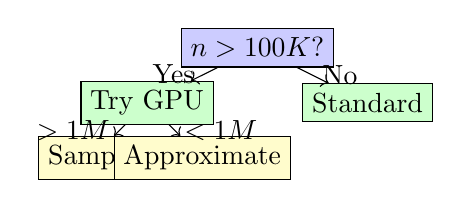
\begin{tikzpicture}[scale=0.7]
\node[draw, fill=blue!20] (root) at (0,0) {$n > 100K$?};
\node[draw, fill=green!20] (gpu) at (-2,-1) {Try GPU};
\node[draw, fill=green!20] (std) at (2,-1) {Standard};
\node[draw, fill=yellow!20] (sample) at (-3,-2) {Sample};
\node[draw, fill=yellow!20] (approx) at (-1,-2) {Approximate};

\draw[->] (root) -- node[left] {Yes} (gpu);
\draw[->] (root) -- node[right] {No} (std);
\draw[->] (gpu) -- node[left] {$>1M$} (sample);
\draw[->] (gpu) -- node[right] {$<1M$} (approx);
\end{tikzpicture}
\end{center}

\textbf{Implementation Libraries:}
\begin{itemize}
\item \texttt{openTSNE}: All methods
\item \texttt{FIt-SNE}: FFT acceleration  
\item \texttt{RAPIDS}: GPU implementation
\end{itemize}
\end{columns}
\end{frame}

% New Slide 63 (Replaces old 71-75)
\begin{frame}{Numerical Stability and Validation}
\textbf{Critical Implementation Details:}

\begin{columns}
\column{0.5\textwidth}
\textbf{Common Numerical Issues:}
\begin{itemize}
\item \textbf{Overflow:} Use log-sum-exp trick
\item \textbf{Division by zero:} Add $\epsilon = 10^{-12}$
\item \textbf{Gradient explosion:} Clip gradients to $[-4, 4]$
\item \textbf{Poor initialization:} Multiple restarts
\end{itemize}

\textbf{Validation Best Practices:}
\begin{itemize}
\item Run \textbf{minimum 5 times} with different seeds
\item Report \textbf{stability}: std dev of positions
\item Check \textbf{convergence}: KL divergence plateau
\item Measure \textbf{trustworthiness} at $k=10$
\end{itemize}

\column{0.5\textwidth}
\textbf{Quality Checklist:}
\begin{enumerate}
\item[$\square$] Perplexity tested: 5-50 range
\item[$\square$] Multiple runs performed
\item[$\square$] Trustworthiness $> 0.9$
\item[$\square$] No isolated points
\item[$\square$] Convergence achieved
\item[$\square$] Parameters documented
\end{enumerate}

\warning{Never trust a single t-SNE run!}

\textbf{Reporting Requirements:}
\begin{itemize}
\item State exact parameters used
\item Include convergence plots
\item Show multiple perplexities
\item Provide code/random seeds
\end{itemize}
\end{columns}
\end{frame}

% REPLACE SLIDES 76-80 WITH THESE 3 SLIDES

% New Slide 76 (Combines ethics and limitations more concisely)
\begin{frame}{Critical Limitations and Ethical Use}
\begin{columns}
\column{0.5\textwidth}
\textbf{Fundamental Limitations:}
\begin{itemize}
\item \textbf{Non-deterministic:} Different runs → different layouts
\item \textbf{No absolute positions:} Only relative structure matters
\item \textbf{No cluster sizes:} Visual size $\neq$ actual size
\item \textbf{Parameter sensitive:} Results change with perplexity
\end{itemize}

\textbf{Ethical Responsibilities:}
\begin{itemize}
\item Report \textbf{all} parameters used
\item Show \textbf{multiple} runs (minimum 3)
\item Never cherry-pick best result
\item Acknowledge when patterns unclear
\end{itemize}

\column{0.5\textwidth}
\begin{center}
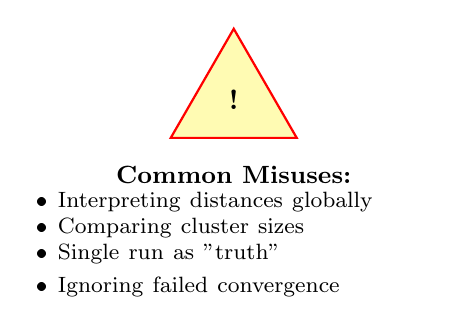
\begin{tikzpicture}[scale=0.8]
% Draw warning triangle
\draw[thick, red, fill=yellow!30] (0,0) -- (2,0) -- (1,1.732) -- cycle;
\node at (1,0.6) {\textbf{!}};
\node[below] at (1,-0.3) {\small \textbf{Common Misuses:}};
\node[text width=5cm, below] at (1,-0.7) {\footnotesize
• Interpreting distances globally\\
• Comparing cluster sizes\\
• Single run as "truth"\\
• Ignoring failed convergence
};
\end{tikzpicture}
\end{center}

\vspace{0.3cm}
\ethics{Always provide: data, code, parameters, and multiple visualizations}
\end{columns}
\end{frame}

% New Slide 77 (Condensed test questions - only essential ones)
\begin{frame}{Key Takeaways: Test Your Understanding}
\textbf{Five Essential Questions:}

\begin{enumerate}
\item \textbf{Why does SNE fail?}\\
\textcolor{gray}{\small Hint: Think about available area in 2D for different distance scales}

\item \textbf{How does Student-t distribution solve the crowding problem?}\\
\textcolor{gray}{\small Hint: Compare tail behavior to Gaussian}

\item \textbf{What does perplexity actually control?}\\
\textcolor{gray}{\small Hint: Not just "number of neighbors"}

\item \textbf{When should you NOT trust a t-SNE visualization?}\\
\textcolor{gray}{\small Hint: Multiple warning signs exist}

\item \textbf{What's the minimum validation needed?}\\
\textcolor{gray}{\small Hint: Think runs, parameters, metrics}
\end{enumerate}

\vspace{0.5cm}
\begin{center}
\colorbox{green!20}{If you can answer these, you understand t-SNE's core concepts!}
\end{center}
\end{frame}

% New Slide 78 (Final resources and practical summary)
\begin{frame}{Resources and Final Guidance}
\begin{columns}
\column{0.5\textwidth}
\textbf{Essential Resources:}
\begin{itemize}
\item \textbf{Original paper:} van der Maaten \& Hinton (2008)
\item \textbf{Interactive guide:} distill.pub/2016/misread-tsne
\item \textbf{Python:} \texttt{scikit-learn}, \texttt{openTSNE}
\item \textbf{R:} \texttt{Rtsne}, \texttt{tsne}
\item \textbf{GPU:} \texttt{rapids-tsne}, \texttt{tsnecuda}
\end{itemize}

\textbf{Getting Started Checklist:}
\begin{enumerate}
\item Start with perplexity = $n/100$
\item Run at least 3 times
\item Try perplexities: 5, 30, 50, 100
\item Check convergence (1000+ iterations)
\item Validate with known structure
\end{enumerate}

\column{0.5\textwidth}
\textbf{Decision Flowchart:}
\begin{center}
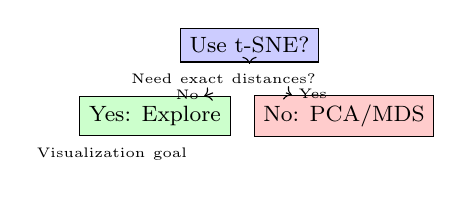
\begin{tikzpicture}[scale=0.6, font=\footnotesize]
\node[draw, fill=blue!20] (start) at (0,0) {Use t-SNE?};
\node[draw, fill=green!20] (explore) at (-2,-1.5) {Yes: Explore};
\node[draw, fill=red!20] (measure) at (2,-1.5) {No: PCA/MDS};
\node[text width=3cm] (q1) at (0,-0.7) {\tiny Need exact distances?};
\node[text width=3cm] (q2) at (-2,-2.3) {\tiny Visualization goal};

\draw[->] (start) -- (q1);
\draw[->] (q1) -- node[left] {\tiny No} (explore);
\draw[->] (q1) -- node[right] {\tiny Yes} (measure);
\end{tikzpicture}
\end{center}

\vspace{0.3cm}
\textbf{Remember:}\\
t-SNE is a \textbf{tool for exploration}, not proof\\
Trust \textbf{consistent patterns} across runs\\
Always \textbf{validate} findings with other methods

\vspace{0.3cm}
\begin{center}
\colorbox{blue!20}{\textbf{Thank you! Questions welcome}}\\
\small Contact: eraco@polytechnic.cat
\end{center}
\end{columns}
\end{frame}

\end{document}